%%% The main file. It contains definitions of basic parameters and includes all other parts.

%% Settings for single-side (simplex) printing
% Margins: left 40mm, right 25mm, top and bottom 25mm
% (but beware, LaTeX adds 1in implicitly)
\documentclass[12pt,a4paper]{report}
\setlength\textwidth{145mm}
\setlength\textheight{247mm}
\setlength\oddsidemargin{15mm}
\setlength\evensidemargin{15mm}
\setlength\topmargin{0mm}
\setlength\headsep{0mm}
\setlength\headheight{0mm}
% \openright makes the following text appear on a right-hand page
\let\openright=\clearpage

%% Settings for two-sided (duplex) printing
% \documentclass[12pt,a4paper,twoside,openright]{report}
% \setlength\textwidth{145mm}
% \setlength\textheight{247mm}
% \setlength\oddsidemargin{14.2mm}
% \setlength\evensidemargin{0mm}
% \setlength\topmargin{0mm}
% \setlength\headsep{0mm}
% \setlength\headheight{0mm}
% \let\openright=\cleardoublepage

%% Generate PDF/A-2u
\usepackage[a-2u]{pdfx}

%% Character encoding: usually latin2, cp1250 or utf8:
\usepackage[utf8]{inputenc}

%% Prefer Latin Modern fonts
\usepackage{lmodern}

%% Further useful packages (included in most LaTeX distributions)
\usepackage{amsmath}        % extensions for typesetting of math
\usepackage{amsfonts}       % math fonts
\usepackage{amsthm}         % theorems, definitions, etc.
\usepackage{amssymb}
\usepackage{bbding}         % various symbols (squares, asterisks, scissors, ...)
\usepackage{bm}             % boldface symbols (\bm)
\usepackage{caption}
\usepackage[aboveskip=2pt]{subcaption}
\usepackage{graphicx}       % embedding of pictures
\usepackage{fancyvrb}       % improved verbatim environment
\usepackage{natbib}         % citation style AUTHOR (YEAR), or AUTHOR [NUMBER]
\usepackage[nottoc]{tocbibind} % makes sure that bibliography and the lists
			    % of figures/tables are included in the table
			    % of contents
\usepackage{dcolumn}        % improved alignment of table columns
\usepackage{booktabs}       % improved horizontal lines in tables
\usepackage{paralist}       % improved enumerate and itemize
\usepackage[usenames]{xcolor}  % typesetting in color
\usepackage{lscape}
\usepackage{listings}
\usepackage[linguistics]{forest}
\forestset{
dg edges/.style={for tree={parent anchor=south, child anchor=north,align=center,base=bottom,where n children=0{tier=word,edge=dotted,calign with current edge}{}}},
}
\usepackage[noabbrev,capitalise]{cleveref}
\usepackage{tikz-dependency}
\usepackage{pgfplots}
\pgfplotsset{compat=1.15}
\usepackage{xspace}

\def\XXX#1{\textcolor{red}{#1}}
\def\hideXXX#1{}
\def\fXXX#1{\XXX{\footnote{#1}}}
\def\furl#1{\footnote{\url{#1}}}
\def\parcite#1{\citep{#1}} % (Smith, 2019)
\def\perscite#1{\citet{#1}} % Smith (2019)
\def\inparcite#1{\citealp{#1}} % Smith, 2019; to be used in parentheses

\def\de2cs{\texttt{de2cs}\xspace}
\def\cs2en{\texttt{cs2en}\xspace}
\def\transformer{Transformer\xspace}
\def\transformerbase{\texttt{Transformer base}\xspace}
\def\transformerrel{\texttt{Transformer relative}\xspace}
\def\seq2seq{\texttt{seq2seq}\xspace}
\def\DiagonalParse{\texttt{DiagonalParse}\xspace}
\def\DepParse{\texttt{DepParse}\xspace}
\def\TreeDistance{\texttt{TreeDistance}\xspace}
\def\TreeTraversal{\texttt{TreeTraversal}\xspace}
\def\SpecPOS{\texttt{SpecPOS}\xspace}
\def\SpecDep{\texttt{SpecDep}\xspace}

%%% Basic information on the thesis

% Thesis title in English (exactly as in the formal assignment)
\def\ThesisTitle{Exploiting Sentence Structure in Neural Machine Translation}

% Author of the thesis
\def\ThesisAuthor{Thuong-Hai Pham}

% Year when the thesis is submitted
\def\YearSubmitted{2018}

% Name of the department or institute, where the work was officially assigned
% (according to the Organizational Structure of MFF UK in English,
% or a full name of a department outside MFF)
\def\Department{Institute of Formal and Applied Linguistics}

% Is it a department (katedra), or an institute (ústav)?
\def\DeptType{Institute}

% Thesis supervisor: name, surname and titles
\def\Supervisor{RNDr. Ond\v{r}ej Bojar, PhD}
\def\SupervisorUni{Charles University in Prague}
\def\CoSupervisor{Dr. Lonneke van der Plas, PhD}
\def\CoSupervisorUni{University of Malta}

% Supervisor's department (again according to Organizational structure of MFF)
\def\SupervisorsDepartment{Institute of Formal and Applied Linguistics}

% Study programme and specialization
\def\StudyProgramme{Informatics}
\def\StudyBranch{Computational Linguistics}


% Abstract (recommended length around 80-200 words; this is not a copy of your thesis assignment!)
\def\Abstract{%
Neural machine translation has been lately established as the new state of the art in machine translation, especially with the Transformer model.
This model emphasizes the importance of the self-attention mechanism and suggests that it can capture some linguistic phenomena.
However, this claim has not been examined thoroughly, so we propose two main groups of methods to examine the relation between the self-attention layer and the ability to capture linguistic information.
Our methods aim to improve the translation performance by directly manipulating the self-attention layer.
The first group focuses on enriching the encoder with source-side syntax with tree-related position embeddings or our novel specialized attention heads.
The second group is a joint translation and parsing model leveraging self-attention weight for the parsing task.
It is clear from the results that enriching the \transformer with sentence structure can help (1).
More importantly, the \transformer model is in fact able to capture this type of linguistic information with guidance in the context of multi-task learning at nearly no increase in training costs (2).
}

% 3 to 5 keywords (recommended), each enclosed in curly braces
\def\Keywords{%
{attention} {machine translation} {dependency} {neural network}
}

%% The hyperref package for clickable links in PDF and also for storing
%% metadata to PDF (including the table of contents).
%% Most settings are pre-set by the pdfx package.
\hypersetup{unicode}
\hypersetup{breaklinks=true}

% Definitions of macros (see description inside)
%%% This file contains definitions of various useful macros and environments %%%
%%% Please add more macros here instead of cluttering other files with them. %%%

%%% Minor tweaks of style

% These macros employ a little dirty trick to convince LaTeX to typeset
% chapter headings sanely, without lots of empty space above them.
% Feel free to ignore.
\makeatletter
\def\@makechapterhead#1{
  {\parindent \z@ \raggedright \normalfont
   \Huge\bfseries \thechapter. #1
   \par\nobreak
   \vskip 20\p@
}}
\def\@makeschapterhead#1{
  {\parindent \z@ \raggedright \normalfont
   \Huge\bfseries #1
   \par\nobreak
   \vskip 20\p@
}}
\makeatother

% This macro defines a chapter, which is not numbered, but is included
% in the table of contents.
\def\chapwithtoc#1{
\chapter*{#1}
\addcontentsline{toc}{chapter}{#1}
}

% Draw black "slugs" whenever a line overflows, so that we can spot it easily.
\overfullrule=1mm

%%% Macros for definitions, theorems, claims, examples, ... (requires amsthm package)

\theoremstyle{plain}
\newtheorem{thm}{Theorem}
\newtheorem{lemma}[thm]{Lemma}
\newtheorem{claim}[thm]{Claim}

\theoremstyle{plain}
\newtheorem{defn}{Definition}

\theoremstyle{remark}
\newtheorem*{cor}{Corollary}
\newtheorem*{rem}{Remark}
\newtheorem*{example}{Example}

%%% An environment for proofs

%%% FIXME %%% \newenvironment{proof}{
%%% FIXME %%%   \par\medskip\noindent
%%% FIXME %%%   \textit{Proof}.
%%% FIXME %%% }{
%%% FIXME %%% \newline
%%% FIXME %%% \rightline{$\square$}  % or \SquareCastShadowBottomRight from bbding package
%%% FIXME %%% }

%%% An environment for typesetting of program code and input/output
%%% of programs. (Requires the fancyvrb package -- fancy verbatim.)

\DefineVerbatimEnvironment{code}{Verbatim}{fontsize=\small, frame=single}

%%% The field of all real and natural numbers
\newcommand{\R}{\mathbb{R}}
\newcommand{\N}{\mathbb{N}}

%%% Useful operators for statistics and probability
\DeclareMathOperator{\pr}{\textsf{P}}
\DeclareMathOperator{\E}{\textsf{E}\,}
\DeclareMathOperator{\var}{\textrm{var}}
\DeclareMathOperator{\sd}{\textrm{sd}}

%%% Transposition of a vector/matrix
\newcommand{\T}[1]{#1^\top}

%%% Various math goodies
\newcommand{\goto}{\rightarrow}
\newcommand{\gotop}{\stackrel{P}{\longrightarrow}}
\newcommand{\maon}[1]{o(n^{#1})}
\newcommand{\abs}[1]{\left|{#1}\right|}
\newcommand{\dint}{\int_0^\tau\!\!\int_0^\tau}
\newcommand{\isqr}[1]{\frac{1}{\sqrt{#1}}}

%%% Various table goodies
\newcommand{\pulrad}[1]{\raisebox{1.5ex}[0pt]{#1}}
\newcommand{\mc}[1]{\multicolumn{1}{c}{#1}}


% Title page and various mandatory informational pages
\begin{document}
%----------------------------------------------------------------------------------------
%	COVER
%----------------------------------------------------------------------------------------
\pagestyle{empty}

\begin{center}

{\huge \bfseries \ThesisTitle\par}
 
\vspace{20mm}

 {\textit \ThesisAuthor}\\
 
\vspace{20mm}

\textsc{MSc. Dissertation}

\vspace{20mm}


\includegraphics[scale=0.15]{img/logo-uom.pdf}

Department of Intelligent Computer Systems\\
Faculty of Information and Communication Technology\\
University of Malta\\
\YearSubmitted

\vspace{20mm}

{Supervisors:} \\
\textit{
    \Supervisor, \SupervisorUni\\
    \CoSupervisor, \CoSupervisorUni
}

\vfill

{Submitted in partial fulfillment of the requirements for the Degree of \\ European Master of Science in Human Language Science and Technology}

\end{center}

\newpage

%----------------------------------------------------------------------------------------
%	DECLARATION PAGE
%----------------------------------------------------------------------------------------
\pagestyle{plain}

\begin{center}

M.Sc. (HLST)\\
\textbf{FACULTY OF INFORMATION AND
COMMUNICATION TECHNOLOGY\\
UNIVERSITY OF MALTA}\\[15mm]

Declaration\\[15mm]

\end{center}

\noindent Plagiarism is defined as “the unacknowledged use, as one’s own work, of work of
another person, whether or not such work has been published” (Regulations
Governing Conduct at Examinations, 1997, Regulation 1 (viii), University of Malta).

\bigskip

\noindent I, the undersigned, declare that the Master’s dissertation submitted is my own work,
except where acknowledged and referenced.

\bigskip

\noindent I understand that the penalties for making a false declaration may include, but are not
limited to, loss of marks; cancellation of examination results; enforced suspension of
studies; or expulsion from the degree programme.
 
\vspace{3cm}

\noindent Student Name: \ThesisAuthor.\\
Course Code: CSA5310 HLST Dissertation.\\
Title of work: \ThesisTitle.\\
\vspace{3cm}

\noindent Signed:\\
\rule[0.5em]{25em}{0.5pt}
 
\noindent Date: \qquad \today\\
\rule[0.5em]{25em}{0.5pt}

\newpage

%----------------------------------------------------------------------------------------
%	ABSTRACT
%----------------------------------------------------------------------------------------

\chapter*{Abstract}

\addcontentsline{toc}{chapter}{Abstract}

\Abstract


%%% A page with automatically generated table of contents of the master thesis

\tableofcontents

%%% Each chapter is kept in a separate file
\chapter*{Introduction}
\addcontentsline{toc}{chapter}{Introduction}

Neural Machine Translation (NMT) has been lately established state of the art in machine translation (MT). To achieve this result, most NMT models highly rely on the attention mechanism \citep{bahdanau:etal:attention:iclr:2015}. It was claimed that this attention mechanism can capture some linguistic structures and phenomena \citep{DBLP:conf/nips/VaswaniSPUJGKP17}. Although \cite{DBLP:conf/acl/BelinkovDDSG17} and \cite{DBLP:conf/emnlp/ShiPK16} had analyzed the amount of linguistic information, POS tags and syntax, respectively, NMT systems could capture, their analyses only applied to systems without attention mechanism. More notably, \cite{DBLP:conf/ijcnlp/GhaderM17} had examined the similarities and differences between attention and alignment matrix. However, their goal was merely to inspect the alignment, not linguistic knowledge in source sentence nor target sentences. Therefore, this thesis is aimed to examine the relevance between linguistic structures, e.g. dependency syntax \citep{melvcuk1988dependency}, and the (self-)attention mechanism (within sentence/self-attention) in NMT, by focusing on two basic questions:
\begin{itemize}
	\item Does explicitly feeding dependency parse to an NMT system help?
    \item If not, is the attention mechanism able to capture these information?
\end{itemize}

\chapter{Theoretical Background}
\label{the}
This chapter presents the basic theories and knowledge that this thesis is built upon.

\section{Machine Translation}
\label{the-mt}

\textit{Machine translation} is an area of computational linguistics aiming to automatically translate text or speech from the \textit{source} language to the \textit{target} language.

Machine translation is distinct from computer-aided translation in which human translators use computer software to support the translation process.
Machine translation should be performed on a fully automatic basis without any human interaction. 
Obviously, a machine translation system can be used during computer-aided translation.

The two most common types of MT system are rule-based and statistical.
These types differ in the way that they are built, but are often combined within the same system which is then called \textit{hybrid MT}.

\textit{Rule-based machine translation (RBMT)} considers language as a set of rules capturing all the relevant regularities in morphology, syntax, or other layers of language description.
In order to translate a sentence, it employs a predefined set of rules within the language to break down the sentence.
Then, another set of rules links between the source and target language, and a robust bilingual dictionary is used to carry out the translation.
These rules are essential for building such a system, but they are usually expensive to construct and must be created anew for each new language pair.

On the other hand, \textit{statistical machine translation (SMT)} does not use linguistic rules to translate but instead a statistical model.
For each unit of the source sentence, there are several possible translations associated with a probability.
% Stress that linguistics *is* usually used when deciding what are the units
The goal of the SMT system is to select these translations for each source unit such that they cover the source sentence with the highest translation probability.
The statistical model helps this selection process, parameters of which must be derived from a sufficient amount of data.
The data in this case is called the \textit{bilingual corpus}, a set of pairs, each consisting of a sentence from the source language and the corresponding sentence in the target language.

From the mid 2010s, the field of MT has seen a new group of systems emerge and then outperform the two previously mentioned types to establish the new state of the art.
These MT systems are actually not too different from SMT as they are also statistical learning models.
However, they employ deep neural networks, which have been very successful in computer vision and simpler linguistic tasks, to model the translation task.
Hence, this type is referred to with a distinct name, \textit{neural machine translation}, which will be discussed in detail in the following section.

\subsection{Neural Machine Translation}
\label{the-mt-nmt}
As mentioned above, a \textit{neural machine translation} system uses a deep neural network to learn the statistical model for machine translation.
Unlike the statistical MT, where all types (word-based, phrase-based or syntax-based) consist of several sub-components that need to be trained separately, NMT can be built and trained in a single neural network.
Such a system is referred to as end-to-end, in which the model is trained at once, directly mapping an input source sentence to its associated sentence in the target language.

The use of neural networks in MT dates back to the works of \cite{Castano97machinetranslation} and \cite{neco1997asynchronous}.
After a break, NMT returned and has started to show promising results with the sequence-to-sequence (\seq2seq) model proposed by \cite{DBLP:conf/nips/SutskeverVL14}.
The idea was based on the assumption that when translating a sentence (in text or speech), a human reads or listens to the whole sentence, understands it, then starts to write down the translated sentence token by token.
Therefore, \seq2seq consists of two main components: an \textit{encoder} and a \textit{decoder} (\cref{fig:seq2seq}).
The encoder consumes the source sentence and produces a fixed-length vector encoding the ``meaning" of the sentence.
This vector is then fed to the decoder.
Finally, the decoder produces the target sentence in the target language token-by-token, based on the context vector and the previously translated tokens. 
In the \seq2seq model, the encoder and decoder are both modelled by a recurrent neural network, or its variant, \textit{long-short term memory} (LSTM) \citep{Hochreiter95longshort-term}.

\begin{figure}
    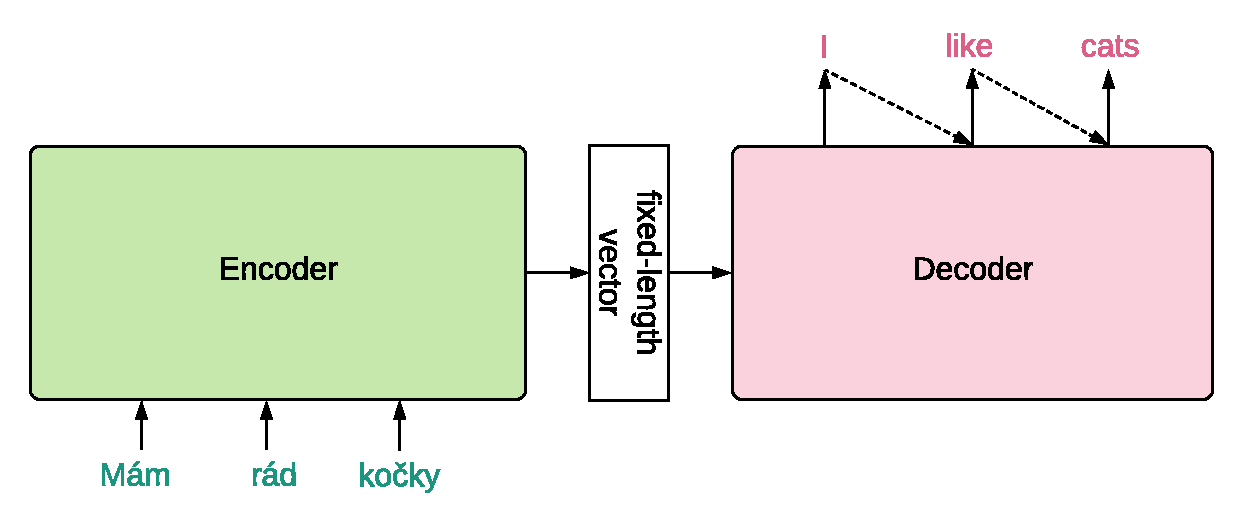
\includegraphics[width=\linewidth]{img/seq2seq.pdf}
    \caption{\seq2seq model.}
    \label{fig:seq2seq}
\end{figure}

\subsection{Attention Mechanism}
\label{the-mt-att}
The assumption that human translators keep in mind the meaning of the entire source sentence is arguable.
Some might argue that the translator has to look back to some part of the source sentence during the translation process.

We are yet to know which is the correct way our brain works during the translation process.
However, from the technical point of view, the limitation of the encoder-decoder approach is that the encoder has to output a fixed-length vector from the source sentence, which is then used in the decoder to output the target sentence.
This means that every decoded token $w$ is condition from the same vector, which captures the whole source sentence, instead of from some parts, e.g. clauses, phrases, etc., of the source sentence which are most associated with $w$.
% This means that all decoded words are based on the same context vector, sentence level instead of the part that gives the most information (clause, phrase, etc.).
In addition, compressing all information into a fixed-length vector leads to the loss of information when the sentence becomes longer.
This is where the attention mechanism is able to help \seq2seq.

\Cref{fig:seq2seq-att} illustrates this mechanism. When translating the second token, the model does not only take into account the information from $s_1$, but also looks back to the encoder. The main computational steps of the attention layer are:
\begin{itemize}
    \item Compute the \textit{attention weights} $a_{2,1}$, $a_{2,2}$, $a_{2,3}$.
    \item Compute the \textit{context vector} $c_2 = a_{2,1}h_1 + a_{2,2}h_2 + a_{2,3}h_3$.
    \item Feed $c_2$ to the computation of $s_2$.
\end{itemize}

\begin{figure}[t]
    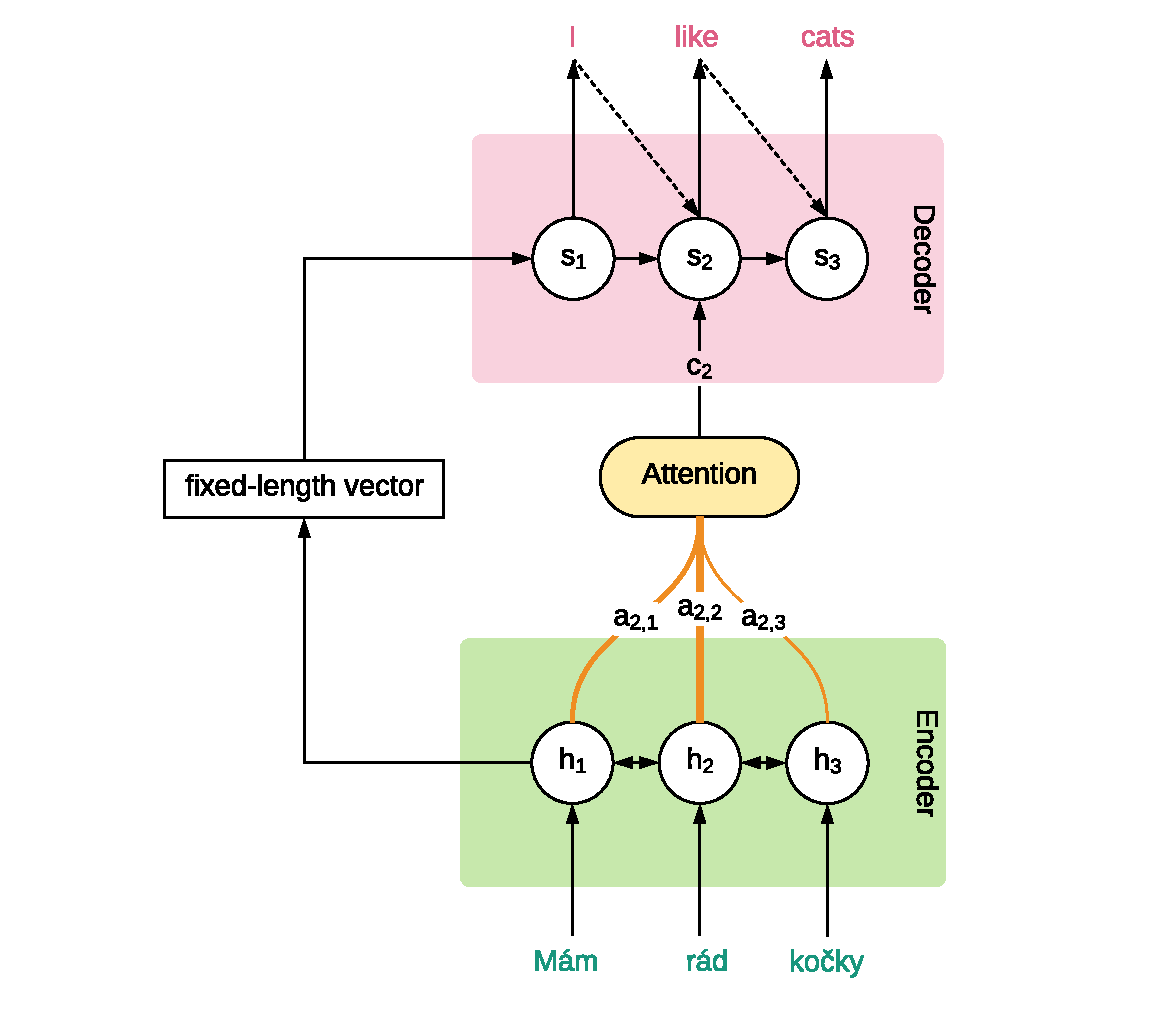
\includegraphics[width=\linewidth]{img/seq2seq-att.pdf}
    \caption{\seq2seq model with Bahdanau attention.}
    \label{fig:seq2seq-att}
\end{figure}


\cite{bahdanau:etal:attention:iclr:2015} proposed the formulas to compute the attention weight $a_{i,j}$ as follows:
\begin{enumerate}
    \item $e_{i,j}=att(s_{i-1}, h_j)$, where $e_{i,j}$ is the \textit{attention energy}, $s_{i-1}$ is the previous hidden state of the decoder, $h_j$ is the hidden state at position $j$ in the encoder.
    \item $a_{i,j}=\frac{exp(e_{i,j})}{\sum_{t}exp(e_{i,t})}$.
\end{enumerate}

The function $att$ is simply a dot product between two vectors. The second step is the \textit{sigmoid function}, ensuring that $\sum_{t}a_{i,t} = 1$, i.e. a distribution. 

This attention mechanism brings a significant improvement to the \seq2seq model.
In some examples, the attention weight matrix is visually similar to the alignment matrix from SMT.
Hence, the attention was also considered as soft-alignment because it does not need to strictly match tokens between the two sentences.

\cite{DBLP:conf/emnlp/LuongPM15} called this type of attention \textit{global attention}, to differentiate from their proposed \textit{local attention}.
In local attention, the attention layer selects one token from the source sentence, then distributes the attention weights, based on a Gaussian distribution, to all neighbors of that token within a fixed-size window.
Due to the considerations of space, we will not elaborate on the local attention, which was discussed by the authors as ``complicated to implement and train".
(see the discussion\footnote{\url{https://github.com/tensorflow/tensorflow/issues/10842\#issuecomment-372546360}} for details).

\section{Evaluation}
\label{the-eval}

In this section, we discuss several methods to evaluate MT systems, which are divided into two types: manual evaluation methods and automatic metrics.

\subsection{Manual Evaluation}
\label{the-eval-manual}
Evaluating MT systems has remained one of the most important problems in the field.
Hence, there are many proposed methods, even on how humans should judge the performance of machine-translated text.
Most of the methods simply judge the hypotheses produced by MT systems, treating the systems as black boxes.

A very straightforward evaluation is to directly assess the adequacy and fluency of whole sentences \citep{DBLP:conf/acllaw/GrahamBMZ13}.
By adequacy, the annotator is expressing to what extent MT captures the meaning of the reference sentence.
Fluency, on the other hand assesses the grammatical correctness and overall quality of the target sentence regardless the source.
In Graham, fluency is merely used to break ties in adequacy.
Another option is to rank full sentences or constituents, i.e. parts of sentences, from several MT systems.
Yet \cite{DBLP:conf/wmt/BojarEPZ11} showed that it is problematic to interpret this manual ranking.

% Comprehension test: Blind editing+correctness check.

As an alternative, task-based methods evaluate if information from MT output is as useful as the original sentence.
Nevertheless, this usefulness is also a vague concept and it is hard to measure.
% Therefore, quiz-based evaluation aims to quantify this problem of task-based evaluation in which given machine-translated snippet, evaluator is asked to answer several questions.

% HMEANT: Is the core event structure preserved? HUME
% Gray-box: Analyzing errors in systems’ output.
% Glass-box: System-dependent: Does this component work?

Although several manual evaluation methods introduced various strategies to overcome the subjectiveness of human judges, this type of evaluation is generally expensive in terms of both time and money.

% One main reason is that the evaluation is not reproducible. 
% Perhaps an even bigger problem is that the evaluation is not reproducible at a small scale.
% • Subjective (some judges are more careful/better at guessing).
% • Not quite consistent judgments from different people.
% • Not quite consistent judgments from a single person!
% • Not reproducible (too easy to solve a task for the second time).
% • Experiment design is critical!

\subsection{Automatic Metrics}
\label{the-eval-auto}

Given the problems of manual evaluation methods described above, it is natural to try to find a fast, cheap, deterministic and replicable metric. Moreover, it would be a plus if the metric allowed automatic model optimization.  

With these properties, the proposed metric can be used to check progress, allow researchers to iterate and evaluate their proposals faster and speed up the development of the field.

The \textit{BLEU} metric (Bilingual Evaluation Understudy, \cite{BLEU}) is one of these automatic evaluation metrics, which is widely used in the field of MT.
It evaluates an output (sentence or corpus) of an MT system (the candidate) by comparing it with correct translations (the references).

The two main components of BLEU are the n-grams precisions and length of the candidate.
Precision is very commonly used in the machine learning field.
In the case of BLEU, it measures the percentage of correct n-grams in the candidate.
The trivial case is unigram ($n=1$) precision which is merely the ratio of the number of tokens shared between candidate and reference divided by the number of tokens in the candidate.
However, this simple definition of precision would not be very precise in some cases, for example:

\bigskip

\textbf{Candidate}: \underline{that} \underline{that} that

\textbf{Reference}: I think \underline{that} it is not \underline{that} bad

\bigskip

The straightforward (lowercase) unigram precision of the above example is 1.0 (100\%), even though only two \textit{that} unigrams in the candidate are matched with the two unigrams in the reference.
That is to say, the number of n-grams shared between the candidate and the reference should be clipped to the number of n-grams that appear in the reference. 
Having that modification, the \textit{modified n-gram precision} in BLEU is computed as follows:

\begin{equation}
    p_n=\frac{\sum_{C\in\{Candidates\}}\sum_{n-gram\in C}Count_{clip}(n-gram)}{\sum_{C'\in\{Candidates\}}\sum_{n-gram'\in C'}Count(n-gram')}
\end{equation}

The second problem BLEU has to deal with is erroneously short candidates.
Take the following example:

\bigskip

\textbf{Candidate}: that

\textbf{Reference}: I think \underline{that} it is not \underline{that} bad

\bigskip

Although the candidate definitely does not express enough information compared to the reference, the precision of this case is $1.0$.
To penalize such output from MT systems, BLEU introduced the \textit{brevity penalty} where $c$ and $r$ are the length of the candidate and the length of the reference, respectively.

\begin{equation}
    BP=\begin{cases} 1 & \mbox{if } c>r \\ e^{(1-r/c)} & \mbox{if } c\le r \end{cases}
\end{equation}

When there are more than one reference, $r$ is called the \textit{effective reference length} and it is taken as the length of the reference that is closest to the length of the candidate.
It is important to note that which reference is the closest varies between implementations of BLEU, see the example below. Both references' lengths are one token different away from the candidate.

\bigskip

\textbf{Candidate}: I like

\textbf{Reference} 1: I like it

\textbf{Reference} 2: I

\bigskip

We advise the reader to use the official BLEU evaluation script used by the Workshop of Machine Translation (WMT) shared task,\footnote{\url{ftp://jaguar.ncsl.nist.gov/mt/resources/mteval-v13a.pl}} or its Python reimplementation.\footnote{\url{https://github.com/mjpost/sacreBLEU}}

Combining those two main components, the BLEU score is defined as follows:

\begin{equation}
    BLEU=BP\cdot exp\left( \sum_{n=1}^{N} w_n \log p_n \right)
\end{equation}

Specifically, BLEU computes the n-grams precisions $p_n$ of the given candidate and references (by default from unigrams to 4-grams).
It then geometrically averages them with predefined weights $w_n$ (all set to $1/4$ by default), and scales down the score in the case of inadequately short candidates with the brevity penalty.

Experimental results showed that BLEU is highly correlated with human evaluators if several reference translations are used and the BLEU scores are sufficiently high \citep{bojar2010tackling}.
However, BLEU is overly sensitive to word forms and sequences of tokens.
There are several proposals to mitigate this, such as using:

\begin{itemize}
    \item Lemmas or deep-lemmas instead of word forms as in SemPOS \citep{Kos09evaluationof}.
    \item Sequences of characters, e.g. chrF3 \citep{chrf3} which is f-score of character 6-grams.
    \item Shorter and gappy sequences, e.g. BEER \citep{beer} uses characters and also pairs of (not necessarily adjacent) words.

\end{itemize}

\section{Linguistic Information}
\label{the-ling}

In this section, we would like to introduce two types of linguistic information that our proposed methods exploit to enhance the translation performance.
\cref{the-ling-dep} discusses the concept of dependency grammar, while \cref{the-ling-pos} reviews various POS tagging systems across languages.

\subsection{Dependency Grammar}
\label{the-ling-dep}

The so-called \textit{dependency grammar} is in fact not a single consistently established grammar but a wide range of variants that share several basic assumptions.
The primary underlying idea is a syntactic structure which consists of lexical items, connected by binary asymmetric relations. 
These relations are called dependencies. 
Although it is said that this concept has been used early in Panini’s work for Sanskrit grammar around the 6\textsuperscript{th} to 4\textsuperscript{th} century BCE, its systematic introduction is due to \cite{lucien1959elements}. 
The two nodes involved in this type of relation are called \textit{head} (\textit{governor})  and \textit{dependent} (\textit{subordinate}).

\begin{figure}
    \centering
    \begin{forest}
    dg edges
    [S
        [NP [I]]
        [VP
            [V [shot]]
            [NP
                [Det [an]]
                [N [elephant]]
                [PP
                    [P [in]]
                    [NP
                        [Det [my]]
                        [N [pajamas]]
                    ]
                ]
            ]
        ]
    ]
    \end{forest}
    \caption{Phrase-structure grammar tree.}
    \label{fig:phrase_structure_tree}
\end{figure}

\begin{figure}
    \centering
    \begin{forest}
    dg edges
    [shot,
      [I [I]]
      [shot]
      [elephant
      	[an [an]]
        [elephant]
        [in
        	[in]
            [pajamas
                [my [my]]
                [pajamas]
            ]
        ]
      ]
    ]
    \end{forest}
    \caption{Dependency grammar tree.}
    \label{fig:dependency_tree}
\end{figure}

In order to visualize these relations in a sentence, a tree-like structure named \textit{dependency tree} is used.
Aside from dependency tree, another common tree-like structure used in describing the grammar of the sentence is the phrase-structure tree.

\cref{fig:phrase_structure_tree,fig:dependency_tree} present an example of a phrase-structure and a dependency tree, respectively.
While the phrase-structure tree represents phrases (as non-terminal nodes) with their structural categories, the dependency tree depicts the head-dependent relations (with directed arcs) between its lexical items.
\cref{fig:dependency_tree_label} also introduces a dependency tree with arc labels, known as \textit{dependency labels}, which specify the functional relation that holds between each pair of lexical items.

In the examples, the noun \textit{elephant} is the dependent of the verb \textit{shot} and the nature of the dependency relation is specified by the label, which indicates that \textit{elephant} is the object of \textit{shot} (\cref{fig:dependency_tree_label}). The phrase-structure tree has a slightly different analysis.
On the 4\textsuperscript{th} level of the tree (\cref{fig:phrase_structure_tree}), the prepositional phrase (PP) is comprised of a preposition (P) and a noun phrase (NP), spanning over the phrase \textit{``in my pajamas"} of the sentence.

\begin{figure}[t]
    \centering
    \begin{dependency}
        \begin{deptext}
        I \& shot \& an \& elephant \& in \& my \& pajamas \\
        \end{deptext}
        \depedge{2}{1}{sbj}
        \depedge{2}{4}{obj}
        \depedge{4}{3}{dmod}
        \depedge{4}{5}{nmod}
        \depedge{5}{7}{pmod}
        \depedge{7}{6}{dmod}
        \deproot{2}{root}
    \end{dependency}
    \caption{Dependency grammar tree with arc labels.}
    \label{fig:dependency_tree_label}
\end{figure}

It should also be pointed out that the convention which two nodes are related, which of them is marked as the dependent and which as the head, and what is the dependency label sometimes varies between treebanks.
For example, the Universal Dependencies 2.0 (UD 2.0, \cite{UD20}) has a different set of labels and sometimes different ways to attach a certain token to its head, than the Prague Dependency Treebanks (PDT, \cite{pdt20:2006}).

\subsubsection{Dependency Parsing}
\label{the-ling-dep-parse}
\textit{Dependency parsing} is a syntactic analysis of lexical items focused on finding the dependency relation between tokens in a sentence.
In other words, dependency parsing is the process that takes a sentence as the input and outputs the dependency tree discussed in the previous section.
The dependency parser can be built using a set of predefined rules or by learning from data.
The dataset that a parser learns from is called a \textit{treebank}.
Data-driven dependency parsing has two prominent approaches: \textit{transition-based} or \textit{graph-based parsing}.

The transition-based parsing maintains a so-called \textit{configuration}. Then, it uses an \textit{oracle} to decide an action, e.g. whether to attach a token to another token, or to change the current configuration. A configuration in a stack-based shift-reduce parser includes:

\begin{itemize}
    \item A \textit{buffer} containing tokens from the input sentence which have yet to be processed.
    \item A \textit{stack} containing all tokens that are being processed.
    \item A \textit{set of dependency relations} where each member is an edge in the final parse tree.
\end{itemize}

The oracle of a transition-based parser is actually a classifier, which can be built with any data-driven approach that can solve a classification problem, for example a neural network \citep{chen2014fast}.
The input of this classifier includes several features extracted from the configuration, while the output is an action from a set of possible actions.
\citeauthor{chen2014fast} proposed a rich set of features including word form, POS tags and currently known arc labels of the top 3 tokens in the stack and the buffer, and also selected children of these tokens.
The main and only component of a transition-based parser that needs to be trained is the oracle.

Compared to transition-based parsing, graph-based parsing is a more direct approach.
Basically, it transforms the problem of dependency parsing to finding the maximum spanning tree in a connected graph.
First of all, a graph-based parser considers all tokens in the sentence as a complete graph.
Utilizing the linguistic information of the tokens, e.g. word forms, lemmas, part-of-speech tags (\cref{the-ling-pos}), etc., the parser predicts the weight of each possible directed edge $(u,v)$, which indicates the likelihood that token $u$ is the head of token $v$.
The parser then finds the maximum spanning tree from the graph based on the computed probabilities.
This maximum spanning tree is the optimal parse tree of the input sentence.

The task of assigning a dependency label to each dependency relation (\textit{dependency tagging}) may be performed during the parsing process or after having obtained the dependency tree. Nevertheless, we will not elaborate on this task, which is of limited relevance to the present thesis.

\subsection{Part-of-Speech Tagging}
\label{the-ling-pos}

By definition, a \textit{part of speech (POS)} is a category of words that have similar grammatical properties.
If two words are assigned the same POS tag, they have similar grammatical functions in the structure of sentences.

It is important to note that the set of POS tags varies among languages. For example, Vietnamese has the tag of nominal classifiers, which English does not. For English, the POS tags from the Penn treebank project \citep{Marcus93buildinga} are commonly used (\cref{tab:penn-pos}).

\begin{table}[t]
\small
\centering
\begin{tabular}{| l | l | l |} 
\hline
    No. & Tag & Description \\
\hline
    1. & CC & Coordinating conjunction \\
    2. & CD & Cardinal number \\
    3. & DT & Determiner \\
    4. & EX & Existential there \\
    5. & FW & Foreign word \\
    6. & IN & Preposition or subordinating conjunction \\
    7. & JJ & Adjective \\
    8. & JJR & Adjective, comparative \\
    9. & JJS & Adjective, superlative \\
    10. & LS & List item marker \\
    11. & MD & Modal \\
    12. & NN & Noun, singular or mass \\
    13. & NNS & Noun, plural \\
    14. & NNP & Proper noun, singular \\
    15. & NNPS & Proper noun, plural \\
    16. & PDT & Predeterminer \\
    17. & POS & Possessive ending \\
    18. & PRP & Personal pronoun \\
    19. & PRP\$ & Possessive pronoun \\
    20. & RB & Adverb \\
    21. & RBR & Adverb, comparative \\
    22. & RBS & Adverb, superlative \\
    23. & RP & Particle \\
    24. & SYM & Symbol \\
    25. & TO & to \\
    26. & UH & Interjection \\
    27. & VB & Verb, base form \\
    28. & VBD & Verb, past tense \\
    29. & VBG & Verb, gerund or present participle \\
    30. & VBN & Verb, past participle \\
    31. & VBP & Verb, non-3rd person singular present \\
    32. & VBZ & Verb, 3rd person singular present \\
    33. & WDT & Wh-determiner \\
    34. & WP & Wh-pronoun \\
    35. & WP\$ & Possessive wh-pronoun \\
    36. & WRB & Wh-adverb \\
\hline
\end{tabular}
\caption{List of POS tags used in the Penn treebank project.}
\label{tab:penn-pos}
\end{table}

On the other hand, this small POS tag set is arguably not sufficient for morphologically rich languages such as Czech. 
In the Czech language, a complex system of morphological tags is used.
Each morphological tag is an encoded sequence.
This sequence consists of 15 characters whose functions are described in \cref{tab:czech-pos}.

\begin{table}[t]
\small
\centering
\begin{tabular}{| l | l | l |} 
\hline
    No. & Name & Description \\
\hline
     1 & POS & Part of Speech \\
     2 & SUBPOS & Detailed Part of Speech \\
     3 & GENDER & Gender \\
     4 & NUMBER & Number \\
     5 & CASE & Case \\
     6 & POSSGENDER & Possessor's Gender \\
     7 & POSSNUMBER & Possessor's Number \\
     8 & PERSON & Person \\
     9 & TENSE & Tense \\
     10 & GRADE & Degree of comparison \\
     11 & NEGATION & Negation \\
     12 & VOICE & Voice \\
     13 & RESERVE1 & Unused \\
     14 & RESERVE2 & Unused \\
     15 & VAR & Variant, Style, Register, Special Usage  \\
\hline
\end{tabular}
\caption{15 positions of a morphological tag in the Czech language.}
\label{tab:czech-pos}
\end{table}

The very first position denotes 10 basic POS tags (\cref{tab:czech-pos1}), while the second position adds more details about the POS tags.
Hence, the first two characters of a morphological tag can be considered equivalent to the POS tag in the Penn treebank.

For example, the morphological tag of \textit{rezignoval} in the sentence ``\textit{Myslíš, že tě požádají, abys \underline{rezignoval}?}" is \texttt{VpYS---XR-AA---}, which means:
\begin{itemize}
    \item V: verb.
    \item p: verb, past participle, active.
    \item Y: masculine.
    \item S: singular.
    \item X: any person.
    \item R: past tense.
    \item A: affirmative (not negated).
    \item A: active voice.
    \item The hyphen (-) indicates that information at that position is not applicable.
\end{itemize}

\begin{table}[t]
\small
\centering
\begin{tabular}{| l | l |} 
\hline
    Value & Description \\
\hline
    A & Adjective \\
    C & Numeral \\
    D & Adverb \\
    I & Interjection \\
    J & Conjunction \\
    N & Noun \\
    P & Pronoun \\
    V & Verb \\
    R & Preposition \\
    T & Particle \\
    X & Unknown, Not  Determined, Unclassifiable \\
    Z & Punctuation (also used for sentence boundary and token) \\
\hline
\end{tabular}
\caption{Possible values in the first position of a morphological tag in the Czech language.}
\label{tab:czech-pos1}
\end{table}

\chapter{Literature Review}
\label{lit}

Recent attempts to incorporate linguistic information, especially syntactic information, to NMT systems can be roughly classified into two main categories: enriching the encoder or decoder and multi-task learning.

This chapter is subdivided into three sections: the first two sections \cref{lit-enc,lit-mult} discuss the two main categories mentioned above, and \cref{lit-trans} is dedicated to a more detailed review of our baseline, the \transformer model.

\section{Enriching the Encoder or Decoder}
\label{lit-enc}

The main motivation of these methods is to make syntactic information known to the NMT system with the expectation that it might help to improve translation quality.

A very straightforward method to enrich the encoder with syntax is to input this type of information alongside with the word embeddings.
The \seq2seq model with Bahdanau's attention takes word embeddings as input.
\cite{sennrich2016linguistic} reused this model but replaced the input with the concatenation of word embeddings and linguistic features including lemmas, subword tags, POS tags and dependency labels.
The authors reported a significant improvement over the baseline with this simple approach. 

Also in this direction, \cite{DBLP:conf/acl/EriguchiHT16} combined sequence-based encoder with a tree-based encoder.
This tree-based encoder is a modified version of Tree-LSTM \citep{DBLP:conf/acl/TaiSM15}.
In Tree-LSTM, the hidden state vectors are not passed from left to right, but from children to its parent in a tree (\cref{fig:tree-lstm}).
The tree structure must be fed in together with the sentence.
Hence, the encoder is explicitly aware of the syntactic tree and learns the context vector from it.

\begin{figure}[t]
    \centering
    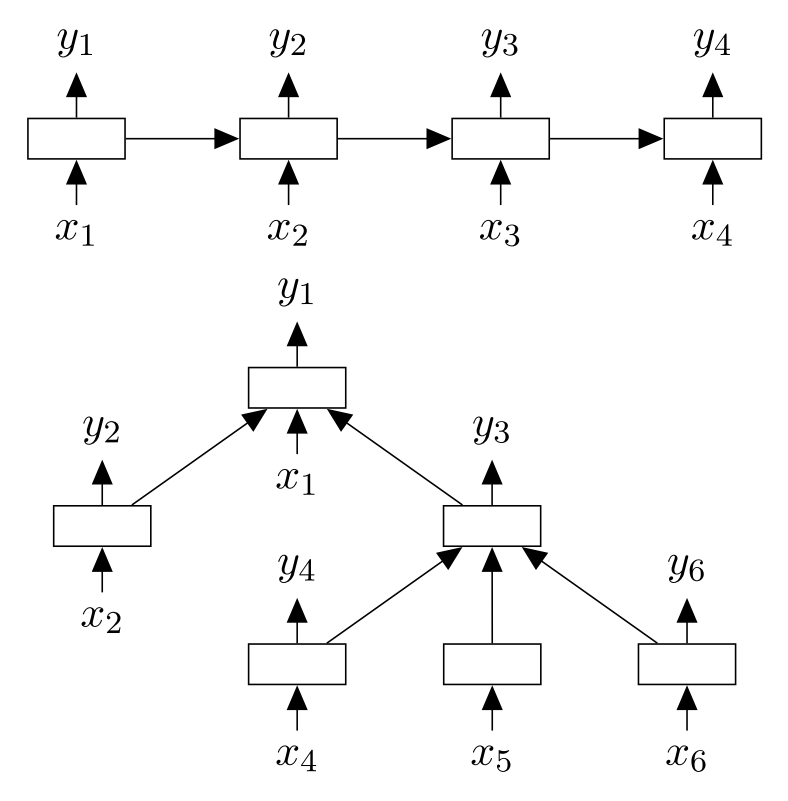
\includegraphics[width=0.7\linewidth]{img/tree-lstm.png}
    \caption{Standard LSTM (top) and tree-LSTM (bottom) (adapted from \cite{DBLP:conf/acl/TaiSM15})}
    \label{fig:tree-lstm}
\end{figure}

In contrast, \cite{DBLP:journals/corr/abs-1711-04231} kept the sequence-based LSTM intact.
However, they replaced the global attention (\cref{the-mt-att}) with their syntax-directed attention.
The proposed attention is analogous to Luong's local attention.
The only difference is how the distance between two words of the source sentence is computed.
In Chen's syntax-directed attention, the distance is the minimum number of edges to be traversed to reach one node from another in the dependency tree.
While in Luong's, it is the sequential distance.

In a simpler way, \cite{DBLP:conf/acl/LiXTZZZ17} proposed to incorporate a sequence of structural label (POS tags) to the encoder's attention by feeding these tags to an RNN.
While not actually focusing on enhancing the encoder, \cite{DBLP:conf/naacl/CohnHVYDH16} introduced structural biases to the encoder-decoder attention function.
These biases include the relative position between the target and source tokens, fertility, Markov condition and bilingual symmetry.
Using this approach, researchers enabled the decoder to attend better to hidden states of the encoder.
It was reported that the proposed approach brought consistent improvements comparing to the attentional model (\seq2seq with Bahdanau's attention).

\section{Multi-Tasking}
\label{lit-mult}

By jointly training the model to parse and translate simultaneously, it is expected that one task can be improved using the knowledge induced from the other task.
\citet{DBLP:conf/acl/EriguchiTC17} combined the translation and dependency parsing tasks by sharing the translation encoder hidden states with the buffer hidden states in a shift-reduce parsing model \cite{DBLP:conf/naacl/DyerKBS16}.

While aiming at the same goal, \citet{DBLP:conf/acl/AharoniG17a} proposed a very simple method.
Instead of modifying the model structure, they represented the target sentence as a linearized, lexicalized constituency tree.
Subsequently, a \seq2seq model was used to translate the source sentence to this linearized tree, i.e. indeed performing the two tasks.
\citet{DBLP:conf/ijcnlp/LeMYM17} made use of the same trick on, however, the dependency tree, proposing a tree-traversal algorithm to linearize the dependency tree.
Unfortunately, their algorithm was not able to traverse a non-projective tree.

The evidence presented in these papers suggests that there is improvement on the BLEU score \citep{BLEU}.
The performance in the secondary task, i.e. parsing, is however not reported.
Going toward the opposite direction, \citet{DBLP:conf/emnlp/ShiPK16} have done an in-depth analysis to further examine the usefulness of NMT model when it came to syntactic parsing. Their work pointed out which type of syntactic relations/labels were better predicted by the \seq2seq MT model.

Aiming to improve both tasks, \cite{tran2018inducing} used two different components in the encoder, one to produce the content and the other to produce the dependency matrix.
While the content is the output of the standard bidirectional LSTM as in the vanilla \seq2seq model, the dependency matrix is produced by a head word selection layer, which is modelled by self-attention (\cref{lit-trans-pos}).
Then both are fed to the decoder using a modified encoder-decoder attentional layer.
In fact, this model is enriching the decoder while still learning to do multi-tasking.

Thus far, most of the multitask models employ another neural network as the parser that is plugged into the NMT system.
Hence, this parser is able to make use of several shared layers with the NMT model.
We would argue that this commonly used setting could hardly answer our question if the translation's encoder is able to capture the source syntax.
The reason is the nature of the input to the parser, which is also the output of the shared layers.
The parser itself is a neural network or another kind of classifier that is complex enough to synthesize lower-level information for its parsing task.
That is to say the input to the parser does not need to be syntactic information.
Therefore, one cannot conclude our second research question even if the parser performs perfectly in the joint model.

In summary, the evidence presented in the literature suggests that various methods to feed syntactic information to NMT helped translation. However, little is known about whether or not NMT already captures syntactic information within the model itself, which is one of the two main questions we attempt to answer with our proposals in the following sections.

\section{The \transformer Model}
\label{lit-trans}

Before starting to discuss our main proposals in the next chapter. We would like to briefly introduce the reader to a novel NMT model that has established the state-of-the-art results in translation - the \transformer model \citep{DBLP:conf/nips/VaswaniSPUJGKP17}.
This model has three interesting features which all of our proposed methods exploit and are built upon: the self-attention mechanism, multi-head attention and the positional encoding.

\subsection{Self-Attention}
\label{lit-trans-att}

The previous studies, reviewed in \cref{lit-enc,lit-mult}, have examined mostly the \seq2seq model with RNNs (LSTMs) as the backbone, whose component is hard to exploit and modify.
The purpose of (bidirectional) LSTMs in the encoder and decoder is to learn the representation of one token using information from its neighbors.
The \transformer model eliminates the need for LSTMs in both encoder and decoder and replaces them with self-attention layers.
These self-attention layers were introduced by \cite{cheng-dong-lapata:2016:EMNLP2016}, which they called intra-attention.
They have been used in natural language inference, sentiment analysis and language modelling.
The \textit{intra-} or \textit{self-} prefixes suggest that this attention mechanism works within the input sentence, instead of between encoder and decoder as in \cref{the-mt-att}. Although the procedures to compute these two types of attention are similar, the attention layer in the \transformer has to perform an additional projection step. 

\cref{fig:self-att-layer} exhibits one typical attention layer in the \transformer, which includes the following steps:
\begin{enumerate}
    \item Project the input $x_i$ to $k_i, v_i, q_i$ using projection matrices $W^K, W^V, W^Q$, respectively.
    \item Compute the attention energy $e_{i,j}$ by a dot product of query $q_i$ and key $v_i$, divided by the dimension $d_k$ of the key.
    \item Compute the attention weight $a_{i,j}=\frac{exp(e_{i,j})}{\sum_{t}exp(e_{i,t})}$.
    \item Compute the output $o_i = \sum_{j} a_{i,j}v_j$.
\end{enumerate}

\begin{figure}[t]
    \centering
    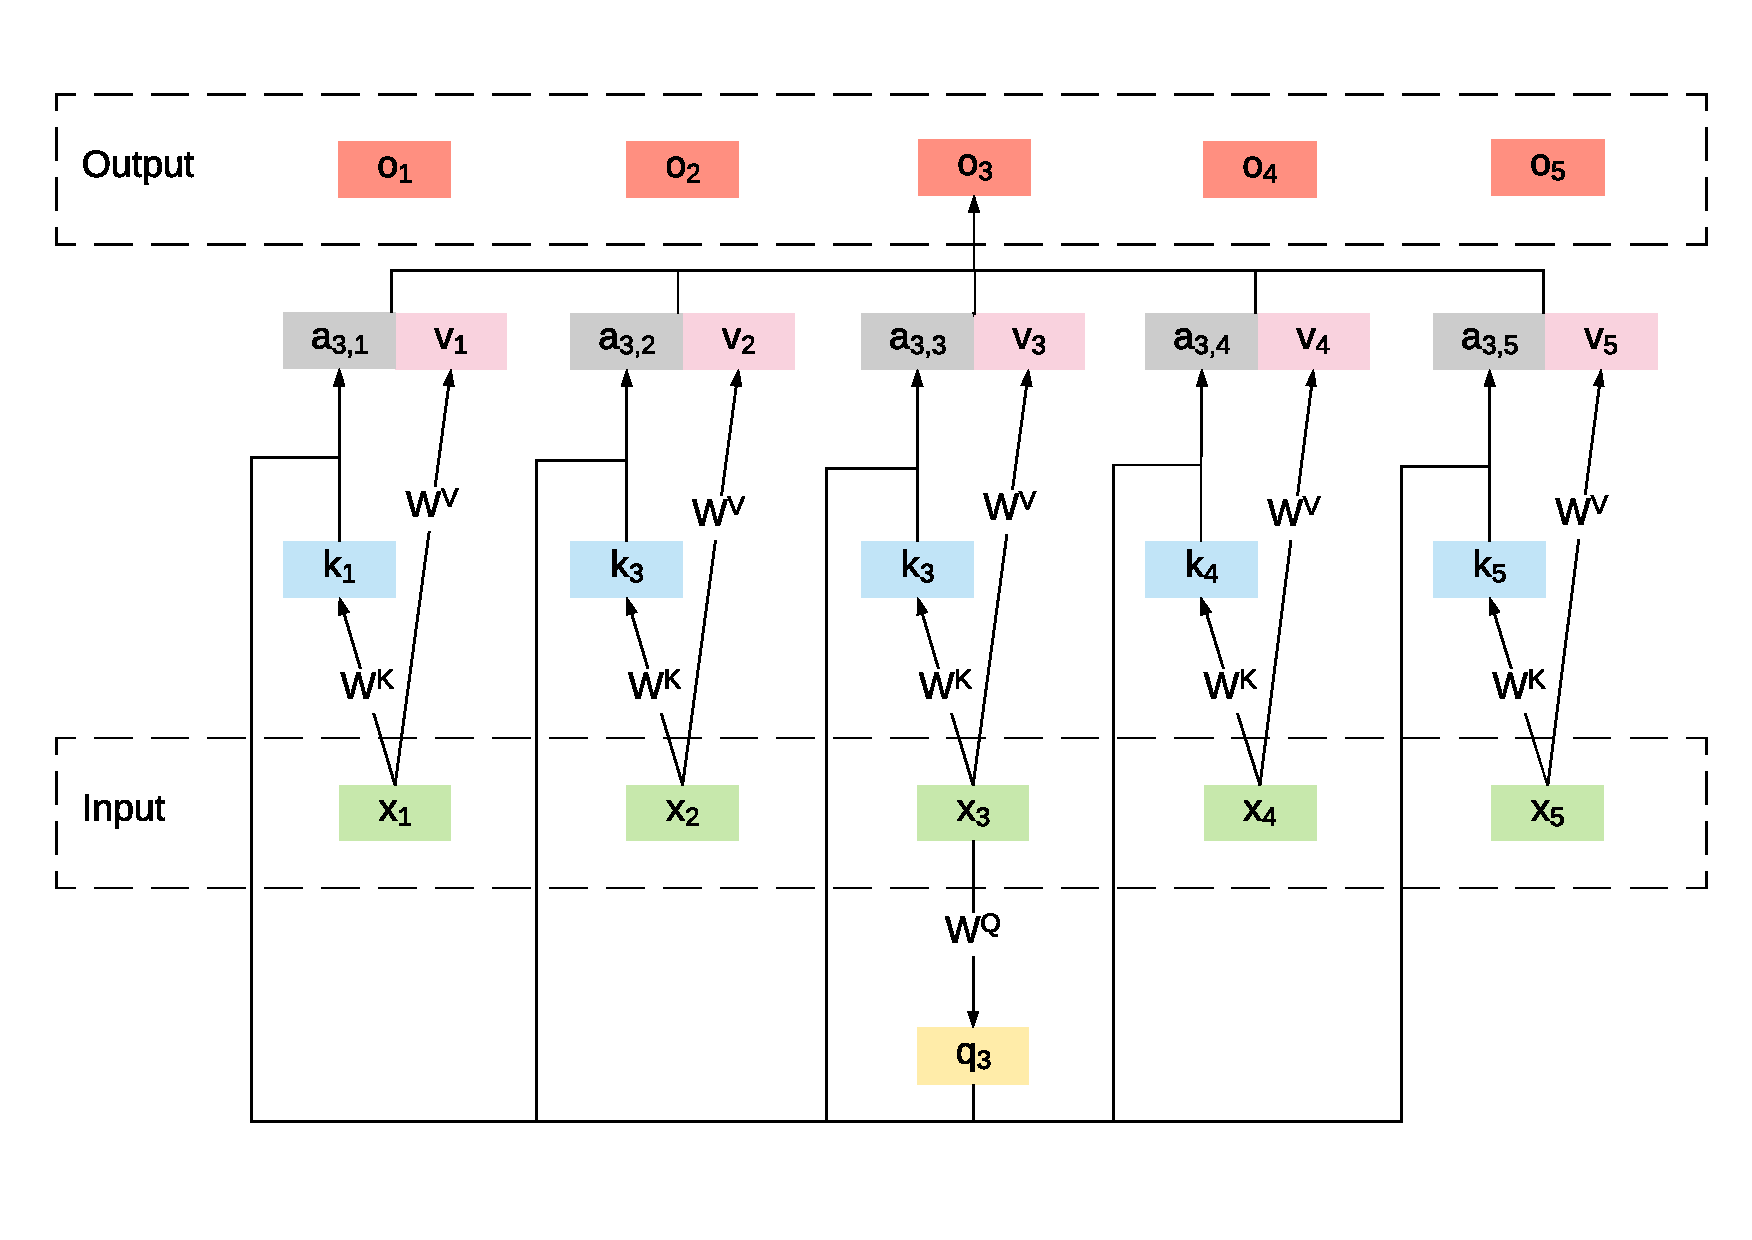
\includegraphics[width=\linewidth]{img/self-att.pdf}
    \caption{A self-attention layer in the \transformer, computing the output $o_3$.}
    \label{fig:self-att-layer}
\end{figure}

\cref{fig:self-att-sample} illustrates an example of attention weight in a self-attention layer.

\begin{figure}[t]
    \centering
    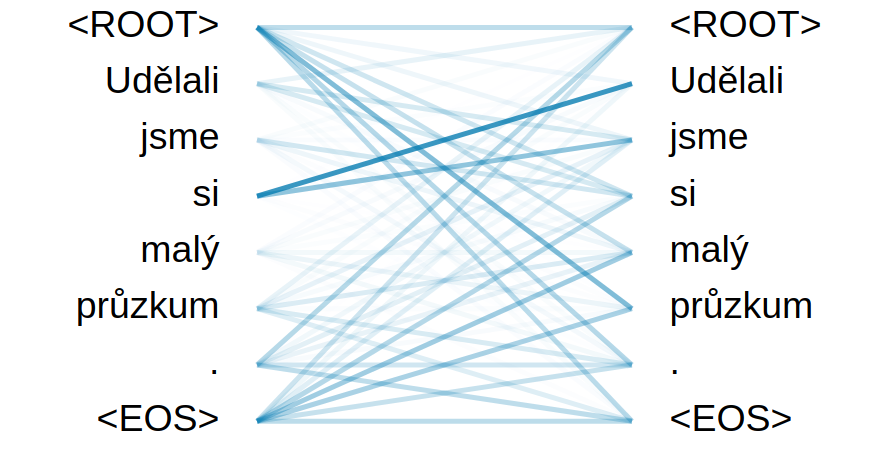
\includegraphics[width=0.6\linewidth]{img/self-att-sample.png}
    \caption{Self-attention example. The visibility of lines denotes attention weight between the layer's output (right) and layer's input (left).}
    \label{fig:self-att-sample}
\end{figure}

One significant advantage of self-attention over RNN is that the network can process in parallel. Parallelization within the layer in RNN is impossible because of the sequential nature of this structure.

\subsection{Multi-Head Attention}

The paper further refined the attention layer by concatenating several attention layers into one ``multi-head attention" layer.
In \cref{fig:multihead-attention-layer}, $h$ independent attention layers are trained in parallel.
The outputs of all are concatenated, then projected through a linear layer.

\begin{figure}[t]
    \centering
    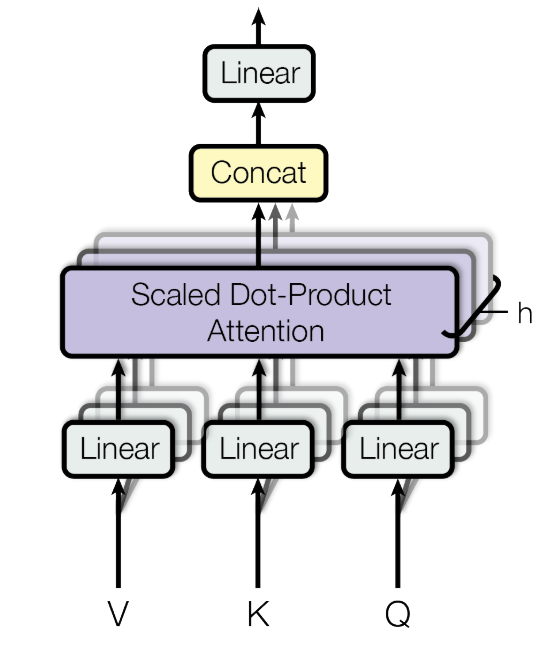
\includegraphics[width=0.5\linewidth]{img/multihead-attention.png}
    \caption{Multi-head attention layer (adapted from \cite{DBLP:conf/nips/VaswaniSPUJGKP17}).}
    \label{fig:multihead-attention-layer}
\end{figure}

This multi-head attention enhances the ability of attention mechanism in two ways:
\begin{itemize}
    \item It makes possible for the model to attend to various information at different positions. Although the attention is able to focus on several positions at one layer, multi-head attention can enable the model to attend to different patterns, and various positions in each patterns.
    For example, a noun in a sentence can attend to all related adjectives in the first attention head. In addition, it can also attend to the pronouns referring it in the second head.
    \item The multi-head attention also allows the keys, queries and values to come from multiple representation subspaces, because of different projection matrices $W^K, W^Q, W^V$ in each head.
\end{itemize}

\subsection{Positional Encoding}
\label{lit-trans-pos}

One prominent problem of replacing LSTMs with self-attention layers is that the model has no notion of token positions.
With the sequential information passing in bidirectional LSTMs, each token is aware of which tokens are before and which are after it.
The self-attention layer simply computes weights using the dot product of tokens' vectors, hence it considers the input as a bag of words.
To deal with this problem, the authors of the \transformer proposed to add a positional embedding vector to each token embedding vector before feeding it to the network.
This positional embedding vector is computed based on the token's position. Specifically, each element $i$ of the vector for the token at position $pos$ is computed by:

\[\begin{cases} \sin\left(\frac{pos}{10000^{i/d}}\right), & \mbox{if } i\mbox{ is even} \\ \cos\left(\frac{pos}{10000^{(i-1)/d}}\right), & \mbox{if } i\mbox{ is odd} \end{cases}\]

in which $d$ is the dimension of the embedding vector.

\begin{figure}
    \centering
    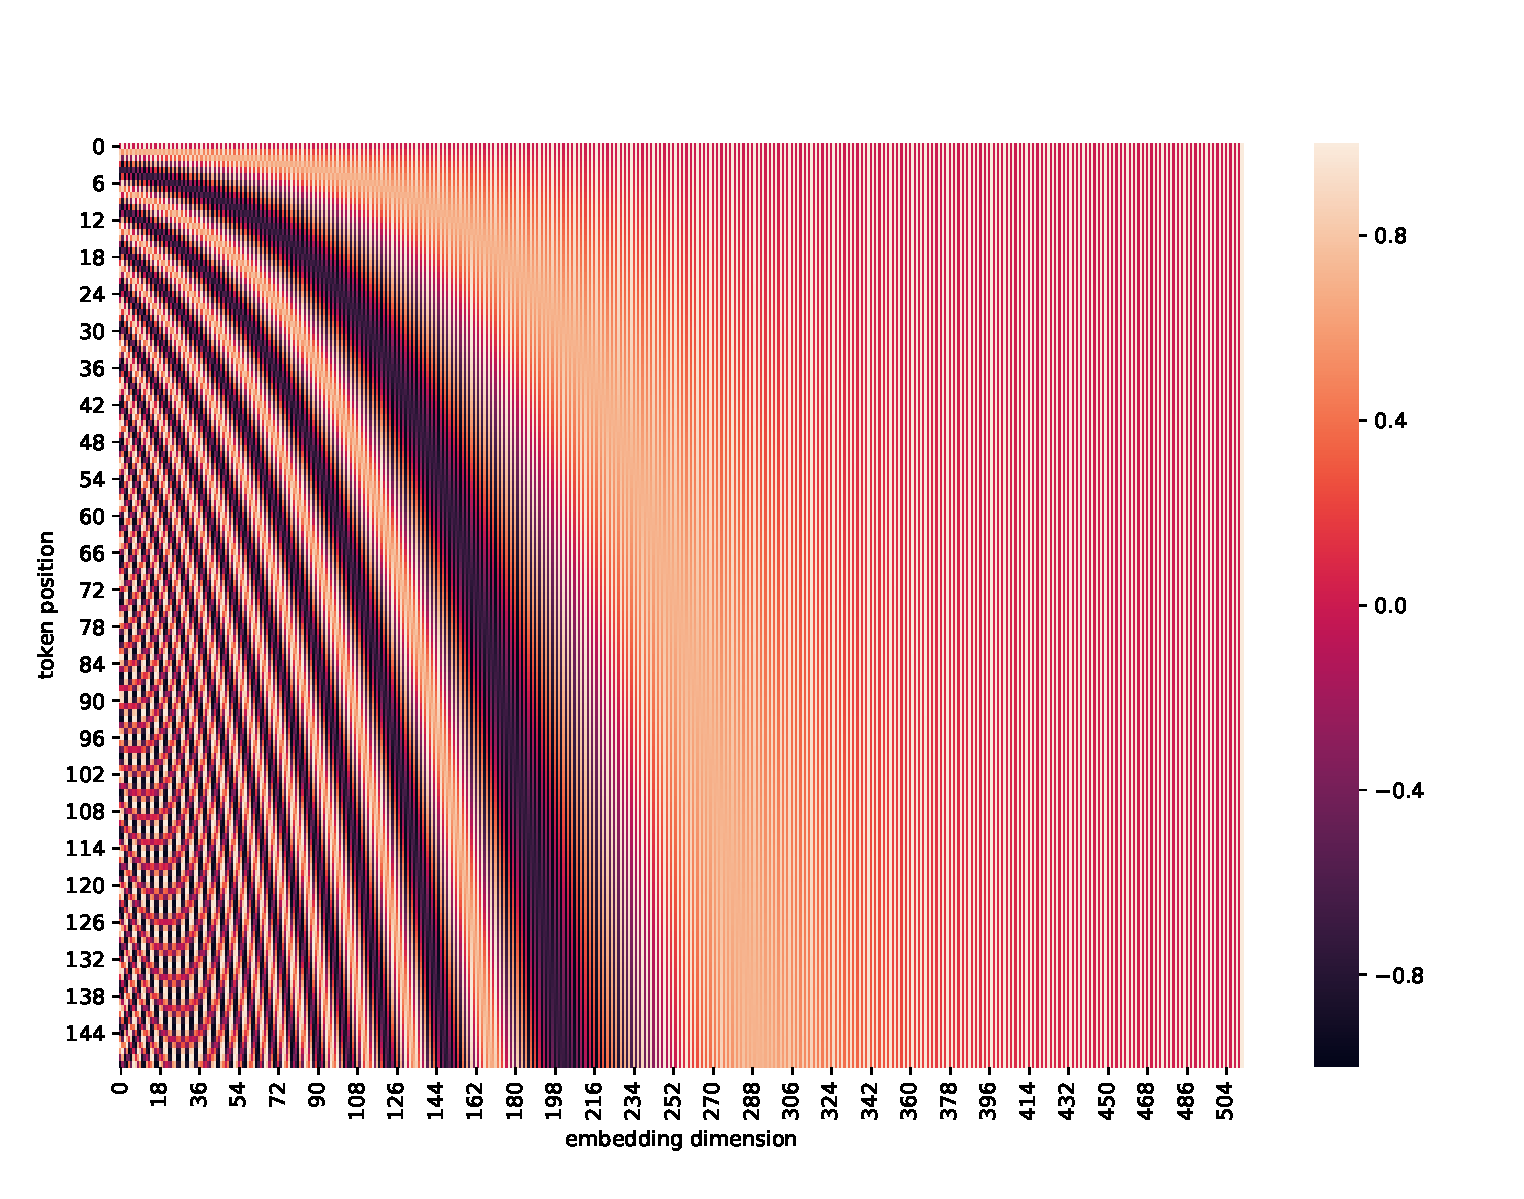
\includegraphics[width=\linewidth]{img/positional-embedding.pdf}
    \caption{Positional embeddings with sine and cosine functions, embedding size $d=512$.}
    \label{fig:positional-embedding}
\end{figure}

\cref{fig:positional-embedding} showcases the values of the generated positional embeddings (dimension of 512) for token positions ranging from 1 to 150.

The authors also experimented with the learned positional embeddings, which were trained in the same manner as word embeddings. It was reported that the two methods yielded comparable results.

\subsection{Model Architecture}
\label{lit-trans-arch}

All the features that we have discussed so far are then used to construct the \transformer model (\cref{fig:transformer}).

\begin{figure}[t]
    \centering
    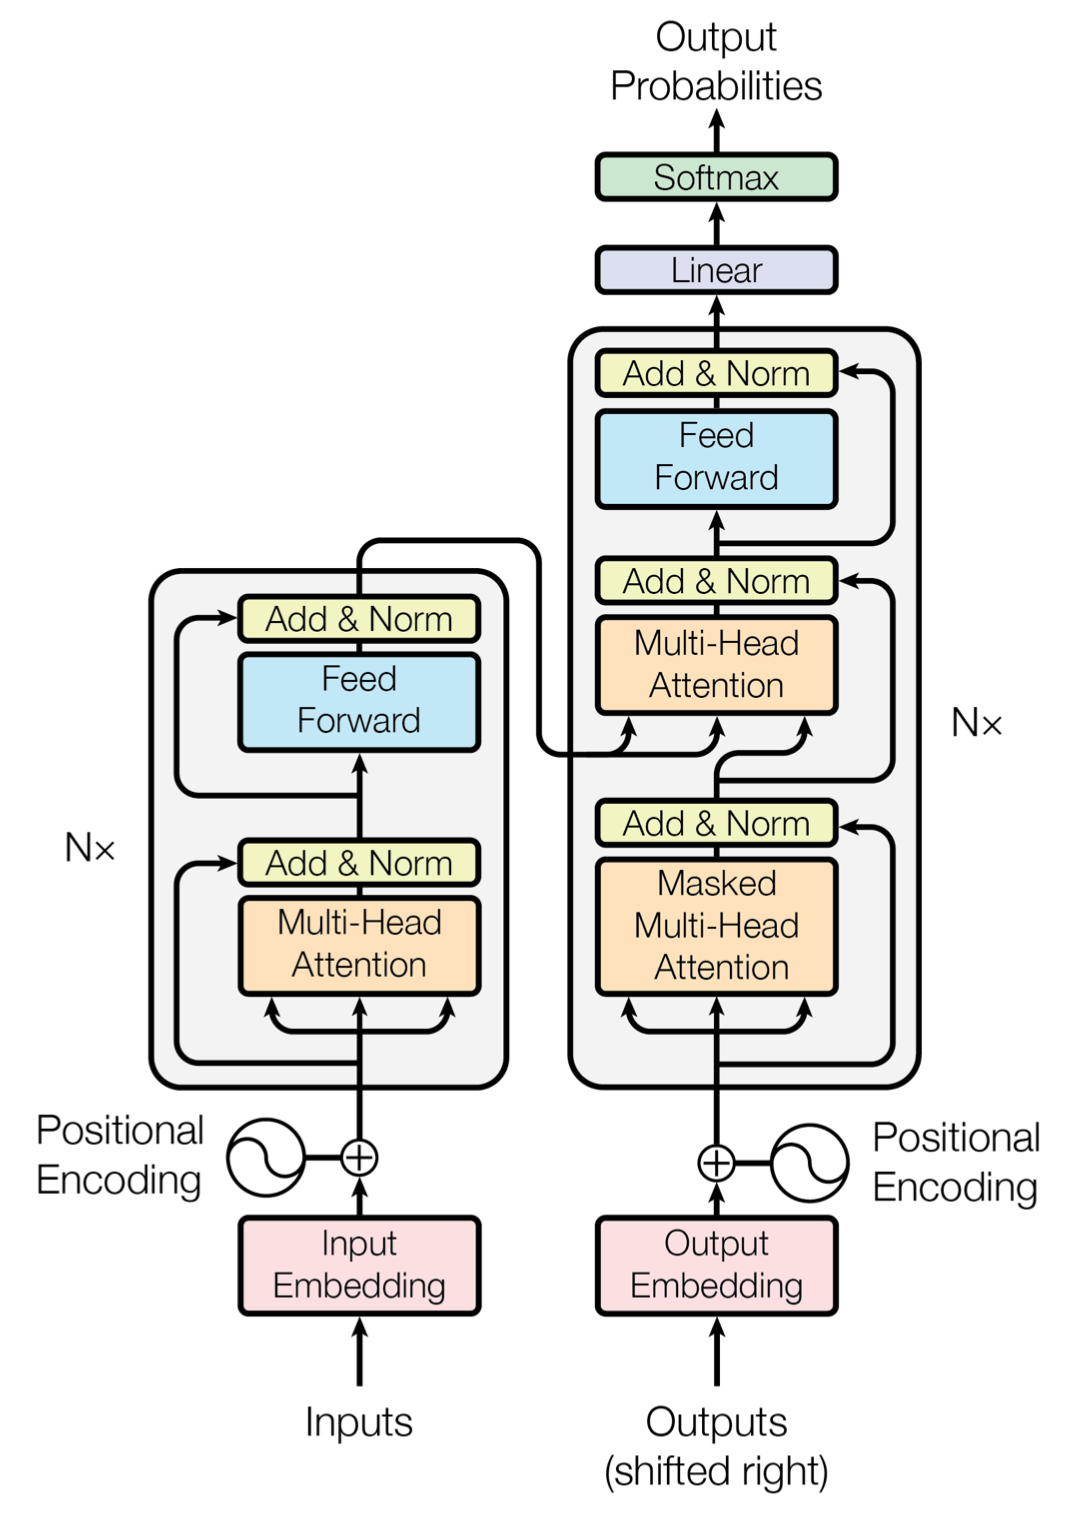
\includegraphics[width=0.9\linewidth]{img/transformer.png}
    \caption{The \transformer model (adapted from \cite{DBLP:conf/nips/VaswaniSPUJGKP17})}
    \label{fig:transformer}
\end{figure}

The model takes the input token embeddings. After being combined with the corresponding positional encoding, they are passed through the encoder, which is a stack of $N$ multi-head attention layers with projection (``feed forward") on top of each.
A similar process applies to the decoder. However, this time the multi-head attention is masked to avoid the attention layer looking into the future, i.e. it should only attend to the tokens translated up to that point.
In addition, between the masked multi-head attention and the projection layer exists another multi-head attention layer. 
This attention layer serves as the encoder-decoder attention in the \seq2seq model.
This is made possible by taking the queries from the output of the decoder's masked attention layer, while the keys and values come from the output of the encoder.
The decoder's output is then passed through another linear projection layer and finally reaches a softmax layer to produce output probabilities.

It is also important to remind the reader that there are several residual connections in \cref{fig:transformer} in which the information flow skips a multi-head attention or feed forward layer and is then recombined with the output of that layer in the ``Add \& Norm" layer.
This ``Add \& Norm" layer also performs the layer-normalization step, which is shown to be useful for the \seq2seq model.\footnote{While its counter-part - the batch-normalization performs well on the computer vision tasks with the convolutional neural network.}

\chapter{Enriching the Encoder by Targeting Self-Attention}
\label{enriching}

In this chapter, we present our proposals to enrich the encoder.
In contrast to \citeauthor{sennrich2016linguistic}, we do not simply feed the network with more information, e.g. POS tags or dependency labels, but directly instruct the self-attention mechanism to build upon these types of information. \cref{enriching-structure} discusses the first approach which introduces dependency-related attentional biases to the \transformer. In \cref{enriching-specialized}, we propose a novel specialized attention head guided by syntactic information.

\section{Structured Attentional Bias}
\label{enriching-structure}

With this approach, we make the \transformer model aware of the source sentence structure by introducing bias terms which are similar to the relative position, but based on the dependency tree.

\subsection{Relative Position}
\label{enriching-structure-relative}

Let us recall the formula to compute the attention energy $e_{ij}$ (before the softmax layer to get attention weight $a_{ij}$):

\begin{equation}
    e_{ij}=\frac{1}{\sqrt{d_k}} x_i W^Q (x_j W^K)^\top
\end{equation}

The energy $e_{ij}$ is simply a dot product of the query $q_i=x_i W^Q$ (input $x_i$ projected through $W^Q$) and the key $k_j=x_j W^K$ (input $x_j$ projected through $W^K$) and divided by the square root of the attention hidden size $d_k$.
The formula above assumes that the positional encoding has been included in the input.
However, this positional encoding is generated from the absolute position of a token within the sentence. \cite{DBLP:conf/naacl/ShawUV18} proposed to impose the encoding of \textit{relative position} in the attention layer instead by adding a bias term:

\begin{equation}
    e_{ij}=\frac{1}{\sqrt{d_k}} x_i W^Q (x_j W^K + b^K_{ij})^\top
\end{equation}

The bias term $b^K_{ij}$ is the embedding vector of the relative position label between token $i$ and $j$. \cref{fig:relative-position-label} illustrates this type of labels between token ``is" and its neighbors in a sample sentence.
These relative position labels are considered as discrete symbols, whose embeddings can be learned the same way as word embeddings.

\begin{figure}[t]
    \centering
    \begin{dependency}
        \begin{deptext}
        I \& think \& this \& is \& a \& good \& idea \& . \\
        \end{deptext}
        \depedge{4}{1}{-3}
        \depedge{4}{2}{-2}
        \depedge{4}{3}{-1}
        \depedge{4}{5}{1}
        \depedge{4}{6}{2}
        \depedge{4}{7}{3}
        \depedge{4}{8}{4}
    \end{dependency}
    \caption{Relative position labels of the token \textit{is} and its neighbors.}
    \label{fig:relative-position-label}
\end{figure}

Following \citeauthor{DBLP:conf/naacl/ShawUV18}, we also enrich the encoder's attention function by introducing structural biases.
Instead of the relative position, we would like to use the information from the source-side dependency tree.
We experiment with two forms of these labels: tree distance and tree traversal encoding.

\subsection{Tree Distance}
\label{enriching-structure-treedist}

Our first proposal is the distance between two nodes in a dependency tree, i.e. the number of edges connecting the two nodes. Our model \TreeDistance utilizes this distance embedding as the bias term $t_{ij}^K$ instead of the relative position bias $b^K_{ij}$, or in a combination of both:

\begin{equation}
 e_{ij}=\frac{1}{\sqrt{d_k}} x_i W^Q (x_j W^K + b^K_{ij} + t_{ij}^K)^\top
\end{equation}

\cref{fig:tree-relative-distance} shows how we obtain the tree distance labels from a dependency tree.
In this example, the distance between \textit{is} and \textit{think} is $1$, because there is one edge connecting them.
On the other hand, \textit{is} and \textit{a} is two edges apart, so the tree distance label is $2$.
It is obvious that this tree distance label is symmetrical, i.e. the tree distance between $i$ and $j$ is identical to the tree distance between $j$ and $i$.

To be able to learn the embeddings, the model has to limit the maximum distance to maintain a fixed-size set of these labels. All token pairs that exceed this maximum distance are assigned a special label, which is similar to the out-of-vocabulary token (\texttt{<OOV>}).

\begin{figure}[t]
    \centering
    \begin{forest}
    dg edges
    [ROOT
        [think, edge={<-}, edge label={node[midway,fill=white] {2}}
          [I, edge={->}, edge label={node[midway,fill=white] {2}} [I]] 
          [think]
          [\textbf{is}, red, edge={<-}, edge label={node[midway,fill=white] {1}}
          	[this, edge={->}, edge label={node[midway,fill=white] {1}} [this]]
            [is]
            [idea, edge={->}, edge label={node[midway,fill=white] {1}}
            	[a, edge={->}, edge label={node[midway,fill=white] {2}} [a]]
                [good, edge={->}, edge label={node[midway,fill=white] {2}} [good]]
                [idea]
            ]
          ]
        ]
        [., edge={->}, edge label={node[midway,fill=white] {3}} [.]]
    ]
    \end{forest}
    \caption{Example of tree distance labels of token \textit{is} and the other tokens in a dependency tree. The arc label expresses the tree distance from \textit{is} to the node at the tail of the arc.}
    \label{fig:tree-relative-distance}
\end{figure}

\subsection{Tree Traversal Encoding}
\label{enriching-structure-treetraversal}

We also expand the simple numerical tree distance above into the tree traversal encoding.
This encoding does not only describe the distance but the path from one node to another.
Our model \TreeTraversal makes use of this encoding the same way the \TreeDistance model utilizes the tree distance label.

\cref{fig:tree-traversal-encoding} elaborates our idea in a more intuitive way.
Let us get back to the token \textit{is}, to traverse from \textit{is} to \textit{ROOT}, we need to go up (\textit{U}) twice. 
Hence, the traversal encoding from \textit{is} to \textit{ROOT} is ``\textit{UU}".
It is important to note that while the tree distance is symmetrical, tree traversal encoding is not.
This is because the direction of the path from \textit{is} to \textit{ROOT} is different from the path from \textit{ROOT} to \textit{is}.

\begin{figure}[t]
    \centering
    \begin{forest}
    dg edges
    [ROOT
        [think, edge={<-}, edge label={node[midway,fill=white] {UU}}
          [I, edge={->}, edge label={node[midway,fill=white] {L}} [I]] 
          [think]
          [\textbf{is}, red, edge={<-}, edge label={node[midway,fill=white] {U}}
          	[this, edge={->}, edge label={node[midway,fill=white] {D}} [this]]
            [is]
            [idea, edge={->}, edge label={node[midway,fill=white] {D}}
            	[a, edge={->}, edge label={node[midway,fill=white] {DD}} [a]]
                [good, edge={->} [good]]
                [idea]
            ]
          ]
        ]
        [., edge={->}, edge label={node[midway,fill=white] {UUD}} [.]]
    ]
    \end{forest}
    \caption{Example of tree traversal encodings of token \textit{is} and the other tokens in a dependency tree. The arc label expresses the tree traversal encoding from \textit{is} to the node at the tail of the arc.}
    \label{fig:tree-traversal-encoding}
\end{figure}

In addition to the two characters `\textit{U}' (up) and `\textit{D}' (down), we also add two special characters to denote the path from the current node to its siblings: `\textit{L}' for its left siblings and `\textit{R}' for its right siblings.
In \cref{fig:tree-traversal-encoding}, the traversal encoding from \textit{is} to \textit{I} is ``\textit{L}" instead of ``\textit{UD}", because \textit{I} is the left sibling of \textit{is}.
Sibling notation takes precedence over `U' and `D' but it is limited to siblings of the current node.

The maximum length of this traversal encoding ($max\_traversal$) is also restricted in order to have a fixed-size vocabulary of the traversal encodings.
% This restriction allows the model learn the embeddings better.
Moreover, the size of the vocabulary generated from our tree traversal does not grow exponentially to $max\_traversal$ because the encoding should be of the shortest path between two nodes in the tree. Hence, all possible encodings can be matched with the following regular expressions:
\begin{itemize}
    \item \textbf{U*D*} : go all the way up (or not) and then down (or not).
    \item \textbf{LD*}      : to the left sibling then down.
    \item \textbf{RD*}      : to the right sibling then down.
\end{itemize}

There is no reason to go down then up (e.g. ``DDDDUU") because a shorter encoding with only `D' characters can encode this path (``DD").

\section{Specialized Attention Heads}
\label{enriching-specialized}

In a normal self-attention layer (\cref{lit-trans-att}), the input $x_i$ is projected through three matrices $W^Q, W^K, W^V$ to obtain the corresponding key, query and value vectors.
The reason for these projections, as discussed in the previous section, is to allow the key, query and value to come from various representation subspaces.

We hypothesize that it may be beneficial for the model that one of these vectors truly come from a known representation space even before the projection.
To be specific, at the shallowest layer (layer 0) of the encoder, we propose the value to be projected from the token embedding (as in the standard \transformer), but the key and query should be projected from some linguistic label embeddings, e.g. POS tags or dependency labels.

As illustrated in \cref{fig:specialized-heads}, the input $x_i$ (token embedding on layer 0) is solely projected to the value vector $v_i$, while the query $q_i$ and key $k_i$ are obtained by projecting an additional input sequence $l_i$ (POS embedding).
Because the attention is guided by this supplementary information $l_i$, we would like to call it a ``specialized attention head".

\begin{figure}[t]
    \centering
    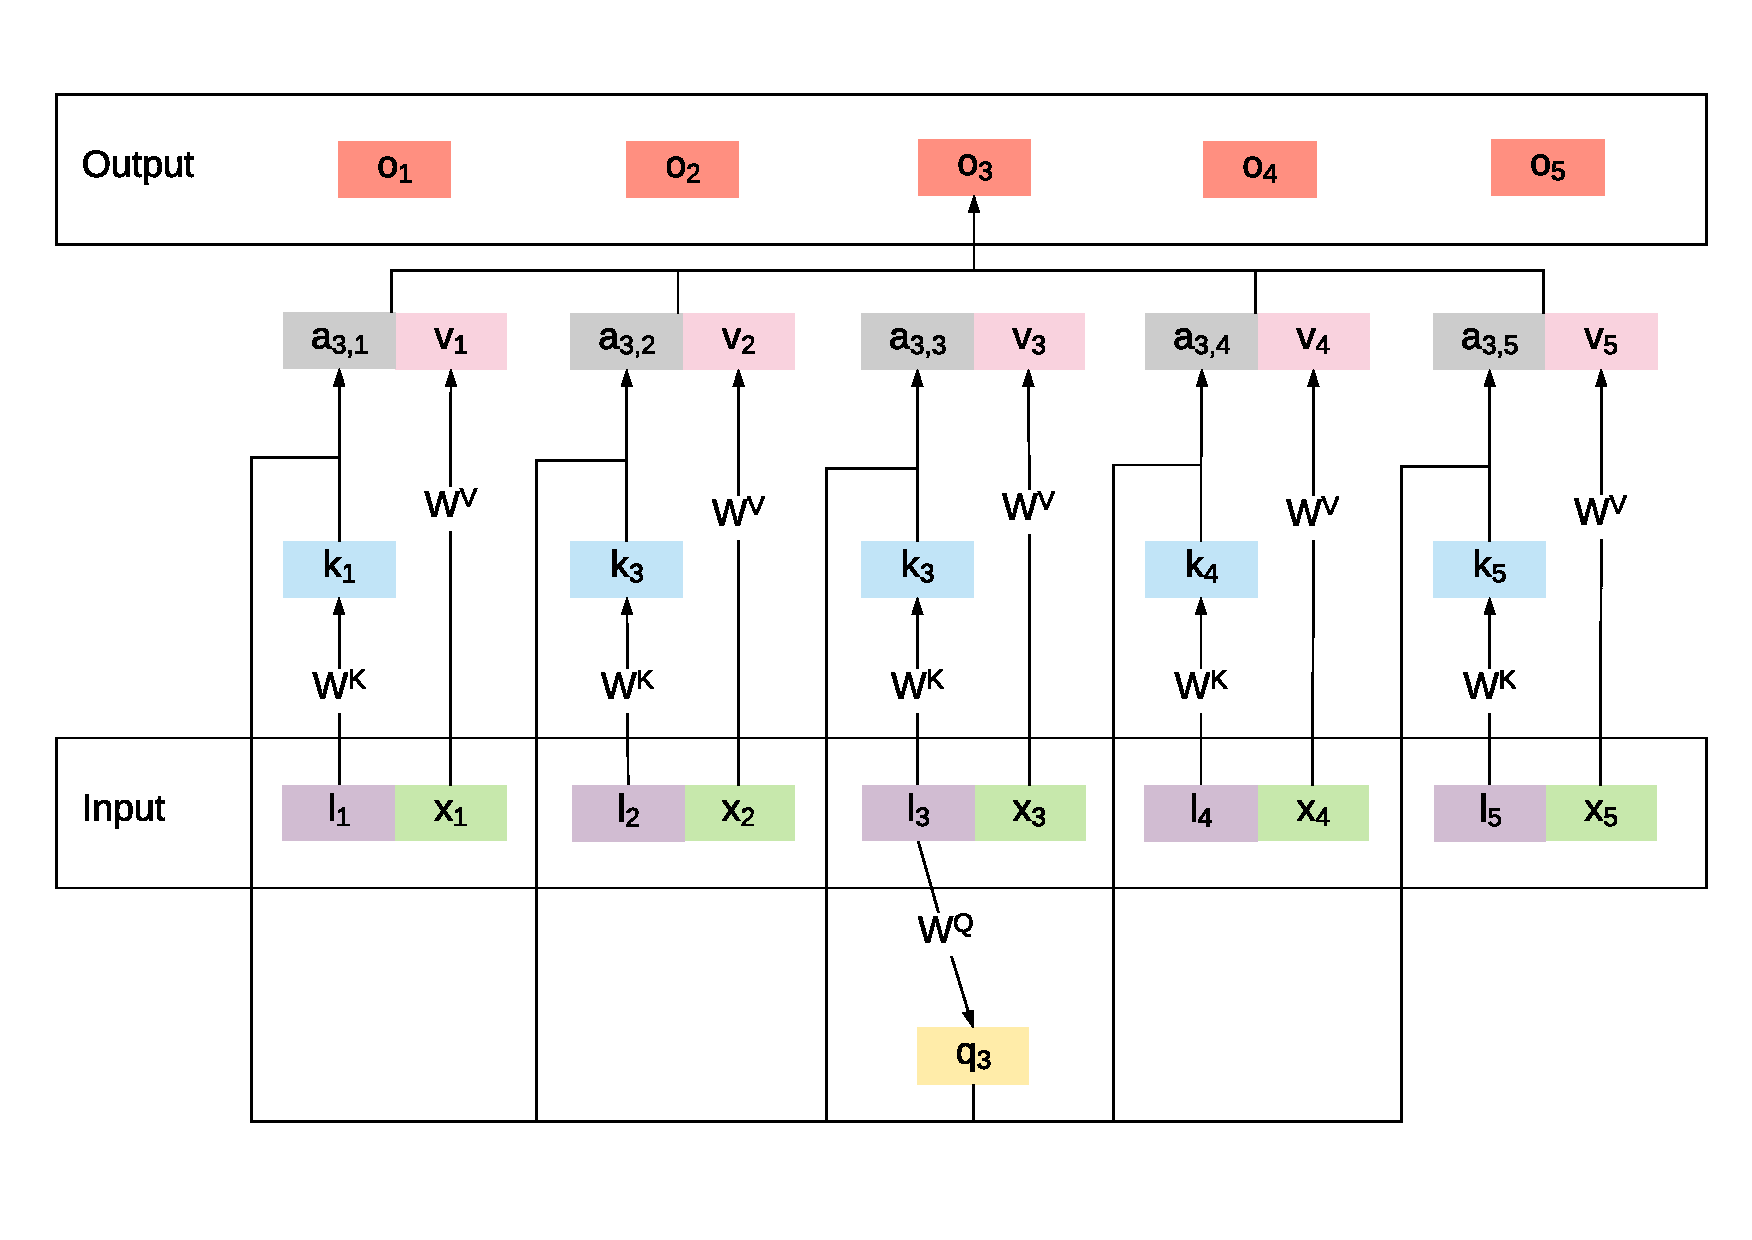
\includegraphics[width=\linewidth]{img/specialized-head.pdf}
    \caption{Specialized attention head with POS tag embeddings as keys and queries, computing the output $o_3$.}
    \label{fig:specialized-heads}
\end{figure}

In our experiment, we only apply this specialized attention in one head of the shallowest layer in the encoder.
In this chosen head, the model will calculate the self-attention weights with keys $k_i$ and queries $q_i$ from one of the following linguistic labels:

\begin{itemize}
	\item POS embeddings (\SpecPOS, \cref{fig:specialized-heads}).
    \item Dependency label embeddings (\SpecDep, $l_i$ is dependency label embedding instead).
\end{itemize}

% instead of token embeddings. Hence, the $l_i$ in \cref{fig:specialized-heads} is either POS tag embeddings or dependency label embeddings.

% \chapter{Multi-task learning with Machine Translation}

% \section{POS Tagging}
% By introducing linguistic information to the model, we hypothesize that the original model was not able to extract this information from raw text, and explicitly feed the model with such information will improve it. However, in the unfortunate event that the translation model has already captured the information of POS tags, it might be helpful to use these attention layers to do POS tagging.

\chapter{Interpreting Self-Attention as Parse}
\label{multitask}

In this chapter, we would like to suggest another set of approaches to multi-task training.
Our proposed approaches attempt to jointly parse the source sentence and translate simultaneously by leveraging the self-attention mechanism in the encoder of the \transformer.
Hence, the model itself can leverage the sentence structure information when translating, and make use of knowledge from translation task during parsing.

\cref{multitask-dep} describes the model that is able to translate and parse the source sentence to produce source dependency tree at the same time.
To examine whether the dependency syntax truly helps translation, we let the model parse a simple sentence structure instead, see \cref{multitask-diagonal}.

\section{Self-Attention as Dependency Parse}
\label{multitask-dep}

Before presenting our proposal in \cref{multitask-dep-parsing}, we would like to briefly introduce a neural dependency parsing model which is our main source of inspiration in \cref{multitask-dep-dozat}.

\subsection{Dependency Parser as Head Selection}
\label{multitask-dep-dozat}

The graph-based dependency parsers, which were discussed in \cref{the-ling-dep-parse}, strive to produce a complete tree structure both during training and inference.
There are also simpler solutions which learn to select the head token of the current token, i.e. head selection, independently.
After the head selection process, a post-editing process handles the output to remove any existing cycle to form a proper tree.
This approach has proven its effectiveness with the neural network model proposed by \cite{dozat:biaffine:2017}.

The model, illustrated in \cref{fig:biaffine-parser}, utilizes two different LSTMs to learn the representation $h^{(arc-dep)}_i$ and $h^{(arc-head)}_i$ for each input $x_i$ independently. This input $x_i$ is a concatenation of the word embedding and POS embedding at position $i$ in the input sentence.
After that, an operation named \textit{biaffine attention} is employed to produce $S_{ij}$ which is the probability that token $i$ is the head of token $j$:

\begin{equation}
    S_{ij} = biaf(h^{(arc-head)}_i, h^{(arc-dep)}_j)    
\end{equation}
where function $biaf$ is a biaffine transformation. All the $S_{ij}$ values form a matrix $S$ which must be column-normalized.
It is then compared against the gold parse tree, encoded as an adjacency matrix (\cref{fig:deptree-vs-matrix}).

In the context of neural networks, the concept of biaffine transformation can be defined, among the commonly used linear transformation and bilinear transformation, as follows:

\paragraph{Linear transformation} is a function $f$ of one variable $x$ ($n$-dimensional), which can be written as 

\begin{equation}
    f(x)=x^\top W
\end{equation}
where $W$ is the parameter of the transformation.

\paragraph{Bilinear transformation} is a function $f$ of two variables $x_1$ and $x_2$ ($n_1$-dimensional and $n_2$-dimensional, respectively), which can be written as 
\begin{equation}
    f(x_1, x_2)=x_1^\top W x_2
\end{equation}
where $W$ is the parameter of the transformation. For any fixed $x_1$, $f(x_1, x_2)$ is linear in $x_2$ and for any fixed $x_2$, $f(x_1, x_2)$ is linear in $x_1$.

\paragraph{Biaffine transformation} is a function $f$ of two variables $x_1$ and $x_2$ (with dimension of $n_1$ and $n_2$, respectively), which can be written as 
\begin{equation}
    f(x_1, x_2) = x_1^\top W_1 x_2 + (x_1\oplus x_2)^\top W_2 + b
\end{equation}
where $x_1 \oplus x_2 $ is the vector concatenation resulting in an $(n_1+n_2)$-dimensional vector. $W_1, W_2$ and $b$ are parameters with the dimensions of $n_1\times n_2$, $n_1+n_2$ and $1$, in that order.

\begin{figure}[t]
    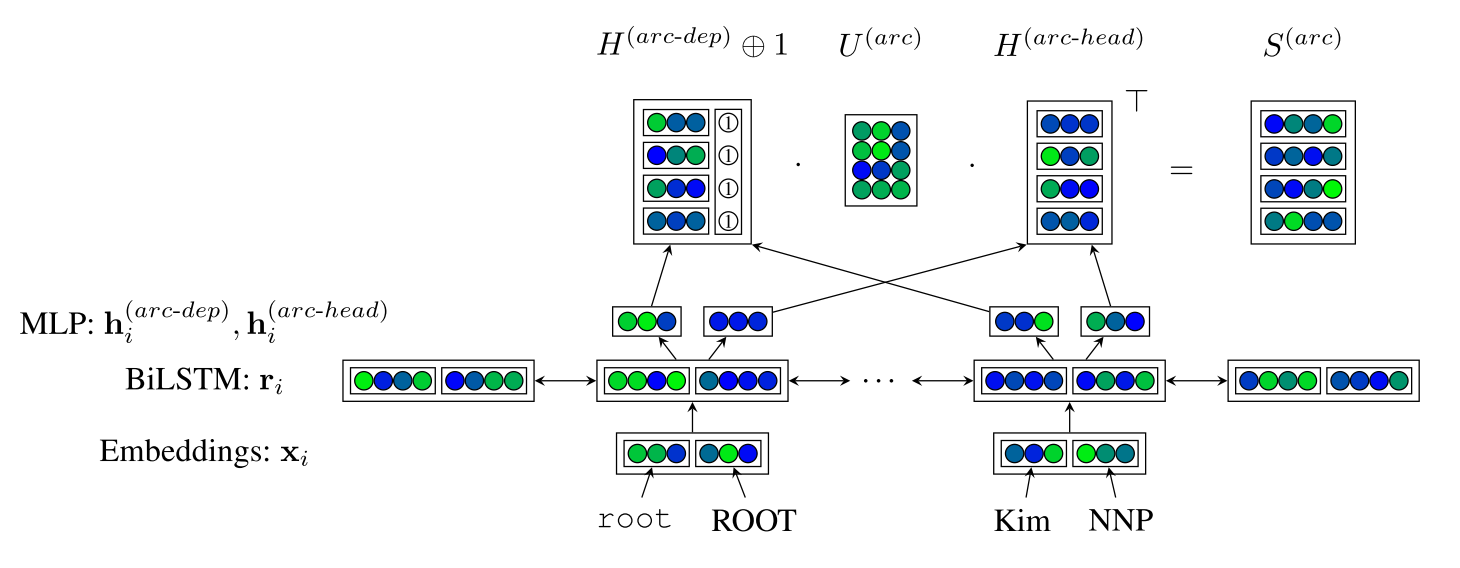
\includegraphics[width=\textwidth]{img/biaffine-parser.png}
    \caption{Neural dependency parser with deep biaffine attention (reproduced from \cite{dozat:biaffine:2017})}
    \label{fig:biaffine-parser}
\end{figure}

\begin{figure}[t]
    \begin{minipage}[b]{0.50\linewidth}
        \centering
        \begin{dependency}[text only label]
            \begin{deptext}
            I \& shot \& an \& elephant \& in \& my \& pajamas \\
            \end{deptext}
            \depedge{2}{1}{}
            \depedge{2}{4}{}
            \depedge{4}{3}{}
            \depedge{4}{5}{}
            \depedge{5}{7}{}
            \depedge{7}{6}{}
        \end{dependency}
    % \rule{6cm}{6cm} %to simulate an actual figure
    \end{minipage}%
    \begin{minipage}[b]{0.50\linewidth}
        \centering
            \begin{tikzpicture}[scale=0.5]
                \draw[step=1cm,draw=gray] (0,0) grid (8,7);
                
                \foreach \f [count=\y] in {I, shot, an, elephant, in, my, pajamas} {
                    \node[left] at (-.2,7.5-\y) {{\raggedleft \f }};
                }
                
                \foreach \e [count=\x] in {ROOT, I, shot, an, elephant, in, my, pajamas} {
                    \node[rotate=60,right] at (\x-.6,7.2) {{\raggedright \e}};
                }
                
                % draw word alignment
                \foreach \x [count=\y] in {2, 0, 4, 2, 4, 7, 5} {
                    \draw[fill=blue!50] (\x,7-\y) rectangle +(1,1);
                }
            \end{tikzpicture}
    \end{minipage}
    \caption{A dependency tree and its representation as an adjacency matrix (the columns represent the heads, the rows are dependents).}
    \label{fig:deptree-vs-matrix}
\end{figure}

\subsection{Parsing from Transformer's Self-Attention Weights}
\label{multitask-dep-parsing}

The construction of the $S$ matrix above is very similar to the matrix of self-attention weights $a_{ij}$ in the \transformer model.
From this similarity, we speculate that the self-attentive architecture of \transformer NMT may have the capacity to learn dependency parsing and we only need to mildly promote the particular linguistic dependencies captured in a treebank. Hence, we could attempt to simulate this parsing model with the self-attention layer in the \transformer model.

\begin{figure}[t]
    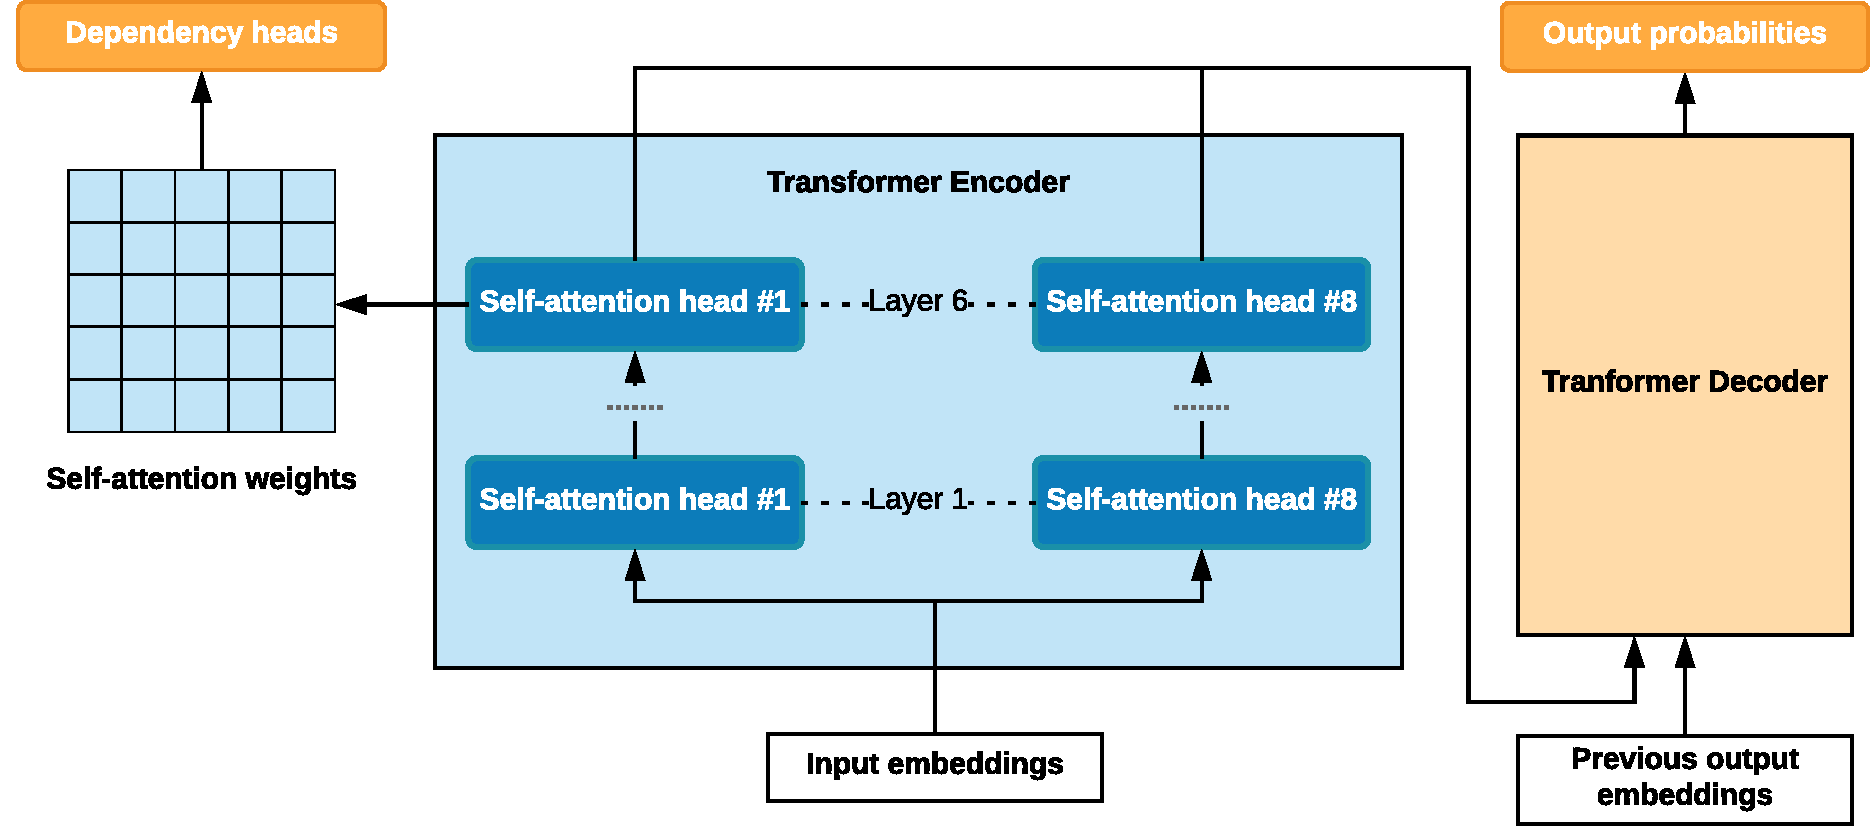
\includegraphics[width=\textwidth]{img/Joint_Translation_DepParse}
    \caption{Joint dependency parsing and translation model (\DepParse and \DiagonalParse).}
    \label{fig:joint_trans_depparse}
\end{figure}

\cref{fig:joint_trans_depparse} illustrates our joint model \DepParse. The translation
part is kept unchanged. The only difference is that we reuse one of the
self-attention heads in the \transformer encoder and reinterpret it as if it was
the dependency matrix $S_{ij}$.
The training objective is combined and
maximizes both the translation quality in terms of cross-entropy of the
candidate translation and the unlabeled attachment score (UAS) of the proposed
heads against the golden parse.\footnote{It should be noted that the dependency
parses we use are actually automatic, produced by
\perscite{mcdonald:pereira:ribarov:hajic:2005} parser incorporated in the Treex
platform, formerly known as TectoMT \parcite{tectomt:popel:2010};
\url{http://ufal.mff.cuni.cz/treex}.}

The particular choice of the head which will serve as the dependency parser is
arbitrary. Put differently, we constrain the \transformer model to use one of its
heads to follow the given syntactic structure of the source sentence. It would be also
possible to use the deep-syntactic parse of the sentence (the
tectogrammatical layer as defined for the Prague Dependency Treebank,
\inparcite{pdt20:2006}); we leave that for future work.

\section{Self-Attention as Diagonal Parse}
\label{multitask-diagonal}

For contrast, we conduct an experiment with a simpler sentence structure, which we call the diagonal parse (dummy dependency parse). In a diagonal parse, the dependency head of a token is simply the previous token (\cref{fig:monotree-vs-matrix}).

Our model for the joint diagonal parsing and translation (\DiagonalParse) is identical to the \DepParse model, which has been described in \cref{fig:joint_trans_depparse}.
For this dummy parsing task, we only need to use diagonal matrices during training instead of the dependency matrices.

The main goal of this method is to examine whether or not the dependency structure really helps or any such constraining of the attention matrix can be beneficial, even a very simple one like the diagonal matrix. 

\begin{figure}[t]
    \begin{minipage}[b]{0.50\linewidth}
        \centering
        \begin{dependency}[text only label]
            \begin{deptext}
            I \& shot \& an \& elephant \& in \& my \& pajamas \\
            \end{deptext}
            \depedge{1}{2}{}
            \depedge{2}{3}{}
            \depedge{3}{4}{}
            \depedge{4}{5}{}
            \depedge{5}{6}{}
            \depedge{6}{7}{}
        \end{dependency}
    % \rule{6cm}{6cm} %to simulate an actual figure
    \end{minipage}%
    \begin{minipage}[b]{0.50\linewidth}
        \centering
            \begin{tikzpicture}[scale=0.5]
                \draw[step=1cm,draw=gray] (0,0) grid (8,7);
                
                \foreach \f [count=\y] in {I, shot, an, elephant, in, my, pajamas} {
                    \node[left] at (-.2,7.5-\y) {{\raggedleft \f }};
                }
                
                \foreach \e [count=\x] in {ROOT, I, shot, an, elephant, in, my, pajamas} {
                    \node[rotate=60,right] at (\x-.6,7.2) {{\raggedright \e}};
                }
                
                % draw word alignment
                \foreach \x [count=\y] in {0, 1, 2, 3, 4, 5, 6} {
                    \draw[fill=blue!50] (\x,7-\y) rectangle +(1,1);
                }
            \end{tikzpicture}
    \end{minipage}
    \caption{Dummy dependencies with diagonal matrix (the columns represent the heads, the rows are dependents).}
    \label{fig:monotree-vs-matrix}
\end{figure}

\chapter{Data and Experiment Setups}

\section{Data}
Experiments in this paper are based on two language pairs: German-to-Czech (de2cs)
translation trained on Europarl \parcite{europarl} and OpenSubtitles2016
\parcite{OPUS}, after some cleanup preprocessing, character normalization
and tokenization. These are the only publicly
available parallel data for this language pair.
Czech-to-English (cs2en) translation was
trained on a subset of CzEng 1.7
\parcite{czeng16:2016}.\footnote{\url{http://ufal.mff.cuni.cz/czeng}}
The data sizes used for MT training are summarized in \cref{tab:data}.
For training on parsing tasks we used the same datasets automatically
annotated on source sides. For German source we used UDPipe \parcite{udpipe},
with model trained on Universal Dependencies 2.0 (UD, \inparcite{UD20}).
For Czech
source we used annotation provided in CzEng release, originally created 
by Treex \parcite{tectomt:popel:2010}. This annotation is based on Prague Dependency Treebank
(PDT, \inparcite{pdt20:2006}). For parsing evaluation we used gold test set from UD
and PDT, respectively.

For Czech-English experiment, we use CzEng 1.7 \citep{czeng16:2016}.

For low-resource language pair, UD pipe with pretrained Parsito model \citep{DBLP:conf/conll/StrakaS17} is used to parse the Estonian-English pair from WMT18 New Translation Task\footnote{http://www.statmt.org/wmt18/}.

\begin{table}
\begin{center}
\small
\begin{tabular}{lrr}
\textbf{Dataset}	& \textbf{de2cs} & \textbf{cs2en} \\
\hline
Train sent. pairs     		& 8.8M      	& 5.2M \\
Train tokens (src/tgt)		& 89M/78M  		& 61M/69M \\
Dev. sent. pairs         	& news 2011: 3k & 1k \\ % test and dev in export format are not available
Test sent. pairs          	& news 2013: 3k & 10k \\
%Source POS tags          	& TreeTagger \parcite{treetagger} & Treex \parcite{tectomt:popel:2010} \\
Dep. parser				  	& UD 2.0 & Treex \\
Gold dep. treebank     & de UD test & PDT test  \\
\end{tabular}
\end{center}
\caption{Data used in our experiments.}
\label{tab:data}
\end{table}

\section{Experiment Setups}

All experiments will use Tensor2Tensor\footnote{https://github.com/tensorflow/tensor2tensor} for model training and visualization.

The seq2seq with Bahdanau attention is chosen to be the baseline for the translation task. While in multi-task learning, each individual model is to be used as baseline for that task.

Experiments in this section were carried out with T2T version 1.5.6 at the
\emph{word level}, i.e. without using subword units. We decided for this
simplification for an easier alignment between the translation and parsing
tasks.

\section{Model Architectures}

The Transformer hyper-parameter set transformer\_base \cite{TrainingTipsfortheTransformerModel} was used for all model variants with hidden size 512, filter size 2048, 8 self-attention heads and 6 layers in each of the encoder and decoder.

We also examined different joint model setups by leveraging the encoder's self-attention weight from various layers (layer 0 to layer 5).

For the preprocessing, the only step needed to be done was to insert a dummy `ROOT' word in the beginning of every sentence, so that the selected self-attention matrix would be able to represent a dependency tree correctly.

\section{Evaluation}

We used BLEU score to automatically evaluate translation task's performance, while unlabeled attachment score is employed for dependency parsing task.

\chapter{Results}
\label{result}

In this chapter, we report the results from all of our experiments and additional observation from the neural network's behavior.
It was reported that choosing a stopping criterion for NMT models is tricky \citep{TrainingTipsfortheTransformerModel} depending on many aspects.
We opted to stop training our models after 500000 steps, at which the \transformerbase was observed to show the sign of convergence.

\section{Enriching Encoder}
\label{result-enriching}

% \cref{tab:res-enriching} reports the results for our effort to enrich the \transformer model.

\subsection{Tree Distance and Traversal}

For the tree distance and tree traversal, it is shown that replacing the positional encoding or relative position with our proposed tree-related encodings does not help the translation.
All of the proposed methods are worse than the baselines.

As listed in \cref{tab:res-enriching}, on the test set, \transformerbase and \transformerrel achieved 36.66 and 37.02 BLEU, respectively, whereas \TreeTraversal, \TreeDistance max 5 and max 20 only got 35.80, 33.13 and 35.50 BLEU, in that order. However, when the tree distance was combined with the positional encoding (\transformerbase) or the relative position (\transformerrel), it yielded better results than both baselines (37.49 and 37.55 vs. 36.66 and 37.02). This is also applied to the case of tree traversal (37.80 vs. 37.02).

\begin{table}[t]
    \begin{center}
    \begin{tabular}{lcc}
        \textbf{Model}        	                            & \textbf{Dev}	& \textbf{Test}	\\
        \hline
        \transformerbase (base)    					        & 37.28 & 36.66 \\
        \transformerrel	(relative)				            & 37.23 & 37.02$^{\dag}$ \\
        \hline
        \TreeDistance, max 5				                & 35.47 & 33.13 \\
        \TreeDistance, max 20				                & 34.45 & 35.50 \\
        \TreeTraversal					                    & 35.21 & 35.80 \\
        (base) + \TreeDistance, max 5					    & 37.67 & 37.49$^{\ddag\blacktriangledown}$ \\
        % (base) + tree distance, max 20					    &  &  \\
        % (base) + tree traversal					        &  &  \\
        (relative) + \TreeDistance, max 20			        & 37.15 & 37.55$^{\ddag\blacktriangledown}$ \\
        (relative) + \TreeTraversal				            & 38.22 & \textbf{37.80}$^{\ddag\blacktriangledown}$ \\
        \hline
        (base) + \SpecPOS						& 36.97 & 36.65 \\
        (relative) + \SpecPOS			& 37.81 & 36.93$^{\dag}$ \\
        (base) + \SpecDep		& 37.53 &  37.72$^{\ddag\blacktriangledown}$ \\
        (relative) + \SpecDep		& 37.66 & \textbf{37.97}$^{\ddag\blacktriangledown}$  \\
    \end{tabular}
    \end{center}
    \caption{Enriching encoder results on \cs2en. Statistical significances are marked as $\dag p < 0.05$ and $\ddag p < 0.01$ when compared to the \transformerbase and $\triangledown/\blacktriangledown$ when compared to the \transformerrel.}
    \label{tab:res-enriching}
\end{table}

\subsection{Specialized Attention Head}

Also in \cref{tab:res-enriching}, for our second approach in the direction of enriching the encoder, the \SpecPOS model, whose one head in layer 0 was chosen to be dedicated as a specialized POS head, could not surpass the baselines (36.65 vs 36.66, 36.93 vs 37.02).

On the other hand, guiding this specialized attention head with dependency label embedding brought $+1.06$ BLEU over the \transformerbase (37.72 vs 36.66).
In addition, \SpecDep when combining with \transformerrel also achieved $+0.95$ BLEU over the \transformerrel (37.97 vs 37.02).

\section{Interpreting Self-Attention as Parse}
\label{result-promote}

\subsection{Diagonal Parsing}
\label{result-promote-diagonal}

Before discussing the result of the parsing tasks (diagonal parsing and dependency parsing), we would like to note that a multi-task model usually requires much longer time to train compared to the single task model, e.g. twice of the training time.
However, all of our multi-task models discussed in this section and the following sections were also trained for only 500000 steps.
The comparison of training time will be reported in \cref{result-speed}.

\cref{tab:res-translate-monoparse} reveals the result of our joint model which is capable of translating and parsing the source sentence to the diagonal matrix.
The diagonal parsing precision is, as expected, very high, from 99.95\% to 99.99\% on the test set.
This joint model also outperformed the baseline in translation task with all of its variants (BLEU scores vary from 37.47 to 38.14, against 36.66).

Moreover, these results form an observable pattern, in which the best result comes from the model which syntax (diagonal matrix) is demanded from the head on layer 0, then the BLEU scores decrease when it come to deeper layers.
We believe a possible explanation for this pattern is because the diagonal matrix represents the relation between the preceding token and the current token.
This is a very simple sentence structure and serves as an additional positional information to the absolute position embeddings.
Therefore, the sooner the model is forced to recognize this information (via training the parsing task), the better it can learn to do translation.

\begin{table}[t]
\centering
\vspace{2ex}
  \begin{tabular}{lcc|cc}
    &  \multicolumn{2}{c}{\textbf{BLEU}} & \multicolumn{2}{|c}{\textbf{Precision}} \\
    & \textbf{Dev} & \textbf{Test} & \textbf{Dev} & \textbf{Test} \\
    \hline
    \transformerbase & 37.28 & 36.66 & -- & -- \\
    \hline
    Syntax demanded from head on layer 0 & 38.68 & \textbf{38.14} & 99.97 & 99.96 \\
    Syntax demanded from head on layer 1 & 39.11 & 38.06 & 99.99 & \textbf{99.99} \\
    Syntax demanded from head on layer 2 & 37.85 & 37.85 & 99.98 & 99.98 \\
    Syntax demanded from head on layer 3 & 37.93 & 37.70 & 99.97 & 99.98 \\
    Syntax demanded from head on layer 4 & 37.68 & 37.47 & 99.98 & 99.96 \\
    Syntax demanded from head on layer 5 & 37.53 & 37.54 & 99.96 & 99.95 \\
  \end{tabular}
  \caption{\DiagonalParse's results in translation (BLEU) and diagonal parsing (precision) on \cs2en. All test BLEU scores are statistical significant with $p<0.01$ when compared to the \transformerbase.}
  \label{tab:res-translate-monoparse}
\end{table}

\subsection{Dependency Parsing}
\label{result-promote-dependency}

Analogous to \cref{tab:res-translate-monoparse}, \cref{tab:res-translate-depparse} presents the results of our joint dependency parsing and translation model.

Let us recall the discussion in \cref{multitask-dep-parsing} that the choice of the head from one layer which will serve as the dependency parse is arbitrary.
However, selecting which layer matters.
In the \transformer's encoder of our experiments, there are six multi-head attention layers.
\cref{tab:res-translate-depparse} shows the result of both tasks when different layers in the encoder were chosen to dedicate one of its self-attention heads to be the dependency matrix.

It is apparent from \cref{tab:res-translate-depparse} that layer 0 (the first layer) was a too shallow layer to demand the syntax from.
Demanding dependency syntax from this layer yielded undesirable results in both translation and parsing task.
The BLEU score of 36.60 is no improvement over the baseline (36.66), while the UAS is at least 8\% lower than other variants of the same model.
We believe this result was caused by the fact that the self-attention mechanism at this layer purely compared between input word embeddings, which perhaps might tend to concern more about lexical meaning than syntax.
Therefore, it could not capture the complex dependency syntax, which is not as simple as the diagonal syntax mentioned in the previous section.
On the other hand, layer 1 performed well on the parsing task (90.78\%), and brought the best improvement to the translation task (38.01).
The translation performance seems to be decreasing when it comes to the deeper layers as well (38.01 - 37.87 - 37.67 - 37.60), which phenomenon we have observed in the diagonal parsing.
The reason, from our point of view, is also similar.
The dependency syntax should be introduced to the model early enough in order to encourage better attention, but not too early.

The performance on the dependency parsing task is shown to behave in the opposite direction.
The UAS values in \cref{tab:res-translate-depparse} are increasing from the shallower to the deeper layer (82.85 - 90.78 - 91.18 - 91.43 - 91.56).
The highest UAS was achieved when the syntax is demanded from layer 4, while the model was still able to maintain good translation performance.
This pattern could suggest that when reaching to the deeper layers, the encoder has already learned a good representation for each tokens.
By good, we mean that the information from other tokens and the relation between those and the current token have been well synthesized by the shallower layers.
Therefore, at these deeper layers, the model can easily infer the dependency syntax.

\begin{table}[t]
\centering
\vspace{2ex}
  \begin{tabular}{lcc|cc}
    &  \multicolumn{2}{c}{\textbf{BLEU}} & \multicolumn{2}{|c}{\textbf{UAS}} \\
    & \textbf{Dev} & \textbf{Test} & \textbf{Dev} & \textbf{Test} \\
    \hline
    \transformerbase & 37.28 & 36.66 & -- & -- \\
    \hline
    Syntax demanded from head on layer 0 & 36.95 & 36.60 & 81.39 & 82.85 \\
    Syntax demanded from head on layer 1 & 38.51 & \textbf{38.01} & 90.17 & 90.78 \\
    Syntax demanded from head on layer 2 & 38.50 & 37.87 & 91.31 & 91.18 \\
    Syntax demanded from head on layer 3 & 38.37 & 37.67 & 91.43 & 91.43 \\
    Syntax demanded from head on layer 4 & 37.86 & 37.60 & 91.65 & \textbf{91.56} \\
    Syntax demanded from head on layer 5 & 37.63 & 37.67 & 91.44 & 91.46 \\
  \end{tabular}
  \caption{\DepParse's results in translation (BLEU) and dependency parsing (UAS) on automatically annotated data (\cs2en). All test BLEU scores, except on layer 0, are statistical significant with $p<0.01$ when being compared to the \transformerbase.}
  \label{tab:res-translate-depparse}
\end{table}

It is important to remind the reader that the parsing results reported up to this moment were computed against the auto-generated treebanks come with the parallel corpus.
Hence, to have a better sense of how our models perform compared to the gold-annotated dataset, we tested our models with the PDT test set for Czech.
The referential parser we used to compare against was from the winner in CoNLL Shared Task 2007 \citep{connl2007}, the latest available evaluation on the same dataset.

In addition to the PDT, we would like to measure the performance on the new annotation convention - the Universal Dependency 2.0. That was the reason we employed our additional dataset \de2cs.
Having discussed in \cref{dataexp-data}, this dataset includes the source trees generated by UDPipe.
Therefore, we selected UDPipe to be the referential parser with this dataset.

\cref{multidec-results} presents the experiment result, in which our proposed
model outperformed the baseline in the translation task on both dataset (14.27 vs. 13.96 and 38.01 vs. 36.66).

\begin{table}[t]
    \begin{center}
    \begin{tabular}{lcc}
        \textbf{Model}        	& \textbf{\de2cs}	& \textbf{\cs2en}	\\
        \hline
        \transformerbase    & 13.96	&  36.66 \\
        \DepParse		& 14.27$^\dag$	&  38.01$^\ddag$ \\
    \end{tabular}
    \end{center}
    \caption{BLEU scores on test sets for translation task ($\dag p < 0.05, \ddag p < 0.01$).}
    \label{multidec-results}
\end{table}

However, in the parsing task against the gold-annotated test sets, \cref{multidec-results-parse} shows that our model achieved better result when parsing on German (de - 81.23 vs. 74.27), but worse on Czech (cs - 82.53 vs 86.28).
An possible excuse is that our model was trained using auto-generated treebanks, not the gold-annotated ones.
Hence, with the current parsing performance, we expect the model to perform better after fine-tuning with the gold-annotated treebanks.

\begin{table}[t]
    \begin{center}
    \begin{tabular}{lcc}
    \textbf{Model}        	& \textbf{de}	& \textbf{cs}	\\
    \hline
    % Stanford \citep{dozat-qi-manning:2017:K17-3} & 84.10 & -- \\
    UDPipe 1.2 (de) 		& 74.27 & -- \\ % UAS: 74.15, LAS: 68.61 in CoNLL Shared task 2017
    Nakagawa (2007) 		& -- &  86.28 \\
    \DepParse			& 81.23 	&  82.53 \\
    \end{tabular}
    \end{center}
    \caption{UAS on the gold-annotated test sets for parsing task.}
    \label{multidec-results-parse}
\end{table}

\subsection{Self-Attention Analysis}
\label{result-promote-analysis}

\begin{figure}[t]
	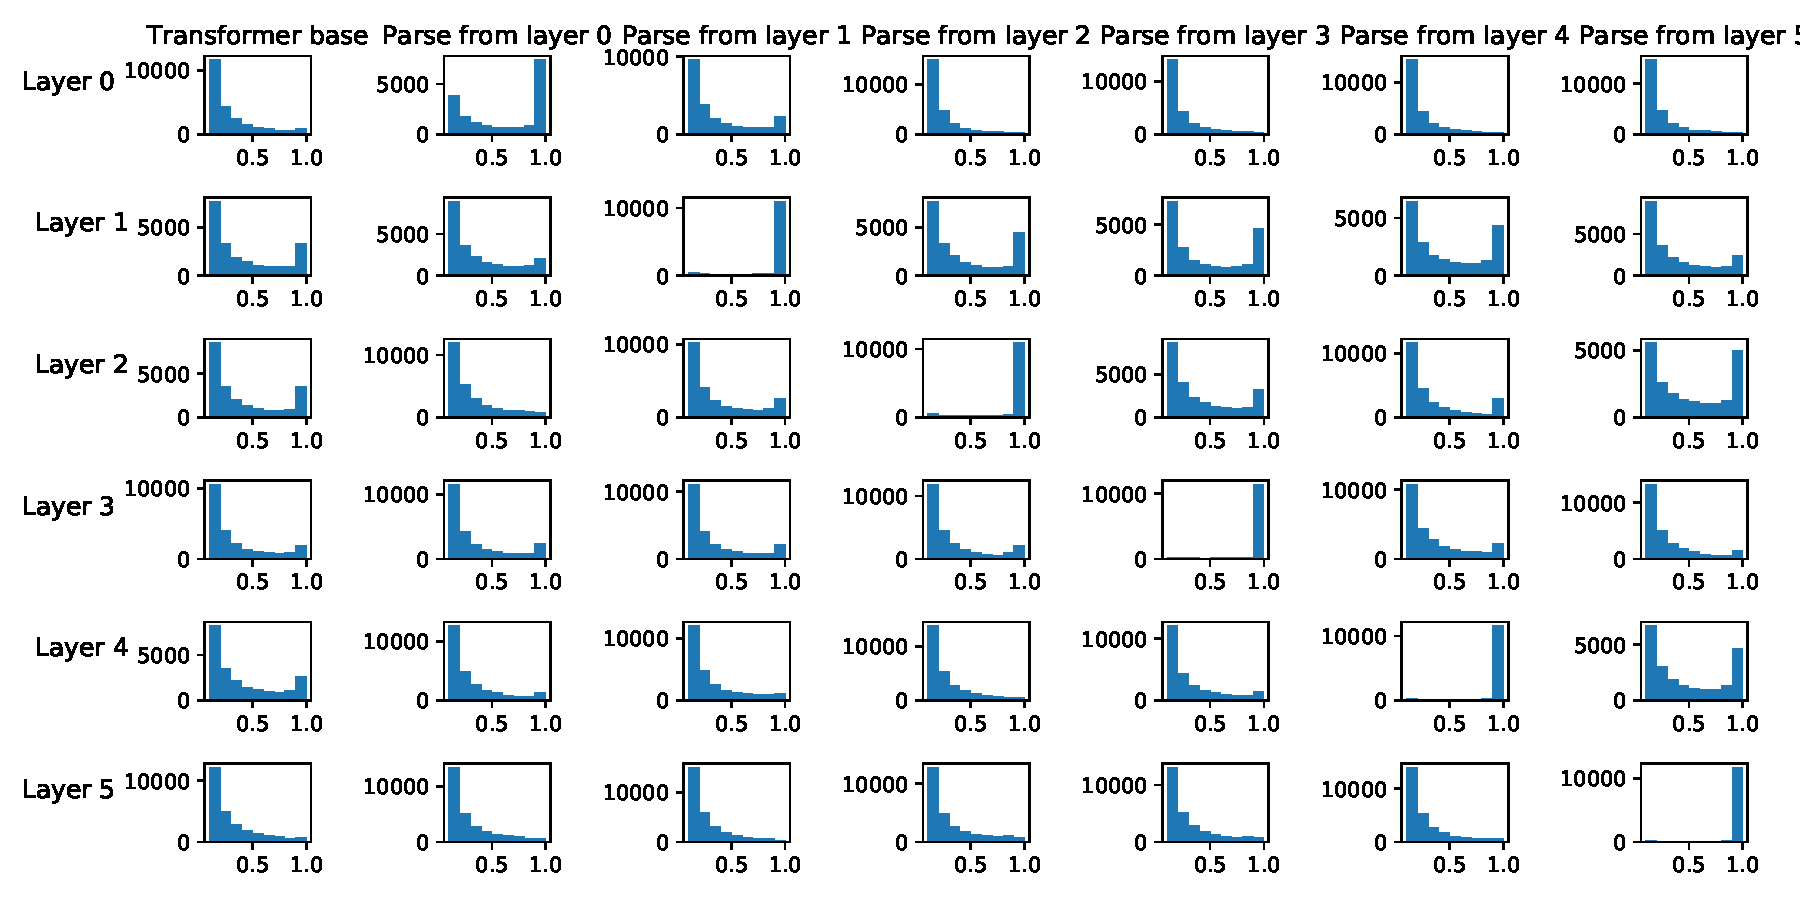
\includegraphics[width=\textwidth]{img/att_dist}
    \caption{Histogram of normalized self-attention weights for each layers (all 8 heads) in the encoder.}
    \label{fig:att_dist}
\end{figure}

In this section, we further analyze the self-attention layers of the \DepParse and \DiagonalParse's encoders in a hope of better understanding the neural network we built.

Figure \ref{fig:att_dist} presents the behavior of self-attention mechanism in each layer of our experimented model that jointly translate and parse dependency tree.
In the figure, while each column represents one variant of our proposed model (except the first column which is the \transformerbase), each row ``Layer $i$" represents the $(i+1)$-th layer in that model.
The histograms were computed after concatenating attention weights from all heads on that layer, and for the first 100 sentences in the \cs2en test set.
In addition, the bin $[0.0,0.1)$ has been removed for better visibility because most of the self-attention weights actually fell into this trivial bin.

As can be seen from the figure, the charts in the diagonal stand out suggests that the chosen layers have very sharp attention distributions, i.e. for each head, the deeper layer attends to only one or two other positions in the shallower layer.
This behavior exists in every one of our multi-task models, except the ``Syntax demanded from head on layer 0".
As mentioned in \cref{result-promote-dependency}, this particular model performed badly on both tasks, hence, our hypothesis is that this sharpness or our restricted self-attention helped the model to perform better.

It is also important to note that one can argue because we used the self-attention weights to predict the dependency heads, it is normal for the head to display this behavior.
However, our analysis suggests that not only the chosen head, but \emph{all} heads in the respective layer also follow this pattern, as revealed in \cref{fig:att_dist_4}.

In \cref{fig:att_dist_4}, the histograms are computed separately for each head on layer 4 (of the model which syntax is demanded from layer 4, bin $[0.0,0.1)$ was also removed).
For \DepParse (\cref{fig:att_dist_4_dep}), it is clearly that not only the chosen head, but other heads in the same layer also have sharp attention distribution.
Similar pattern can also be observed with the case of \DiagonalParse (\cref{fig:att_dist_4_mono}).
We believe the reason for this phenomenon is because of the concatenation and layer normalization after each multi-head attention layer.
The layer normalization over all heads may introduce the sharpness from the chosen head to other heads in the same layer.
We hypothesize that this caused a regularization in the network, which lead to our better performance in translation task.
However, in the scope of this thesis, the exact reason is left for future work.

\begin{figure}[t]
    \centering
    \begin{subfigure}[b]{\textwidth}
	    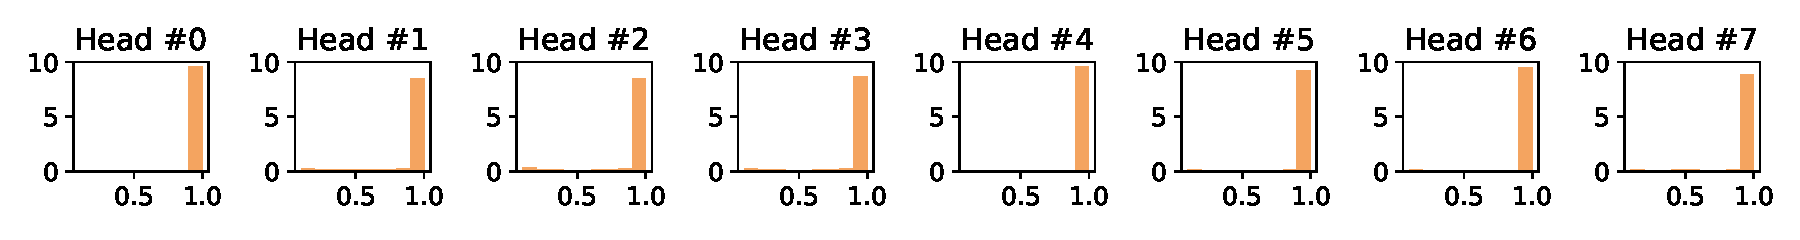
\includegraphics[width=\textwidth]{img/att_dist_4.pdf}
        \caption{\DepParse model.}
        \label{fig:att_dist_4_dep}
    \end{subfigure}
    \begin{subfigure}[b]{\textwidth}
	    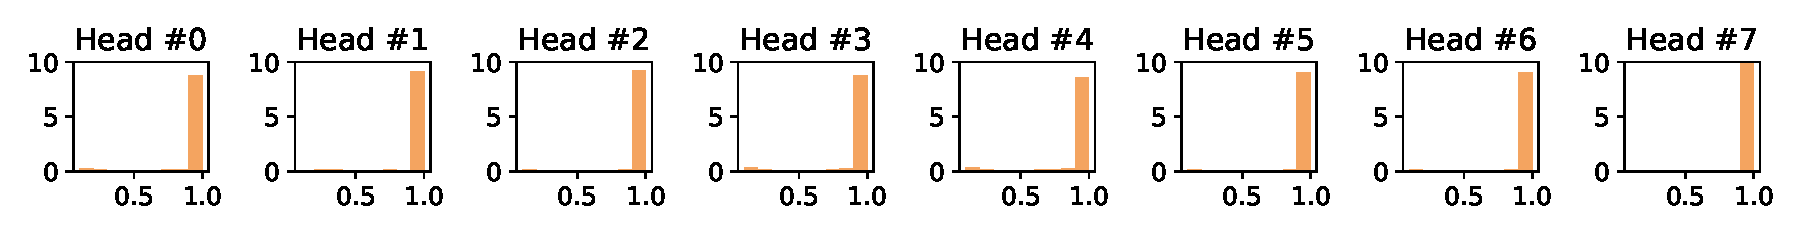
\includegraphics[width=\textwidth]{img/mono_att_dist_4.pdf}
        \caption{\DiagonalParse model.}
        \label{fig:att_dist_4_mono}
    \end{subfigure}
    \caption{Histogram of self-attention weights for each head in layer 4 when demanding the parse tree from layer 4.}
    \label{fig:att_dist_4}
\end{figure}

\cref{fig:att-from4} illustrates the notion of sharpness above in a more intuitive way by visualizing the attention weights for our sample sentence.
The model generated this sample is the \DepParse in which syntax is demanded from layer 4.
Hence, it is obvious that the attention edges on layer 4 are sharper, each token concentrates on a smaller number of tokens in the sentence.
While on the other layers, each token attends to nearly all other tokens in the sentence, with smaller weight for each attention edge.

\begin{figure}[t]
    \centering
    \begin{subfigure}[b]{0.9\textwidth}
        \centering
	    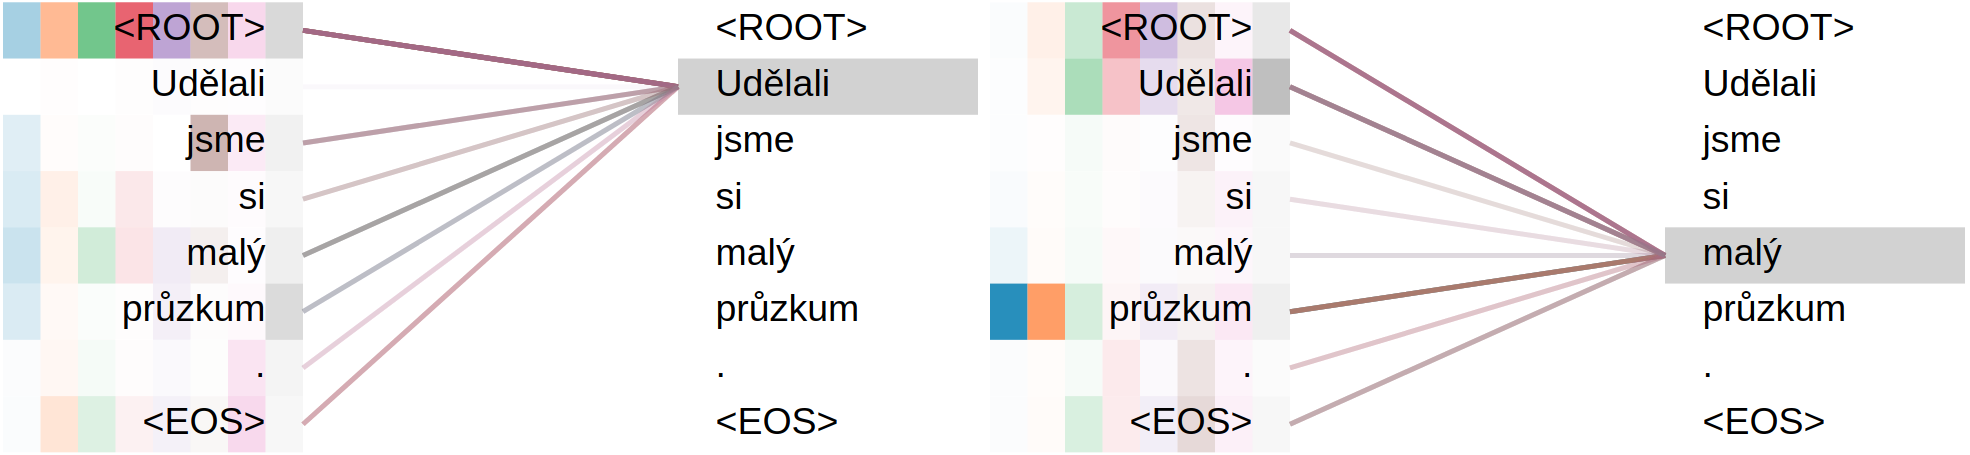
\includegraphics[width=\textwidth]{img/att-from4-l0.png}
        \caption{Layer 0}
    \end{subfigure}
    \begin{subfigure}[b]{0.9\textwidth}
        \centering
	    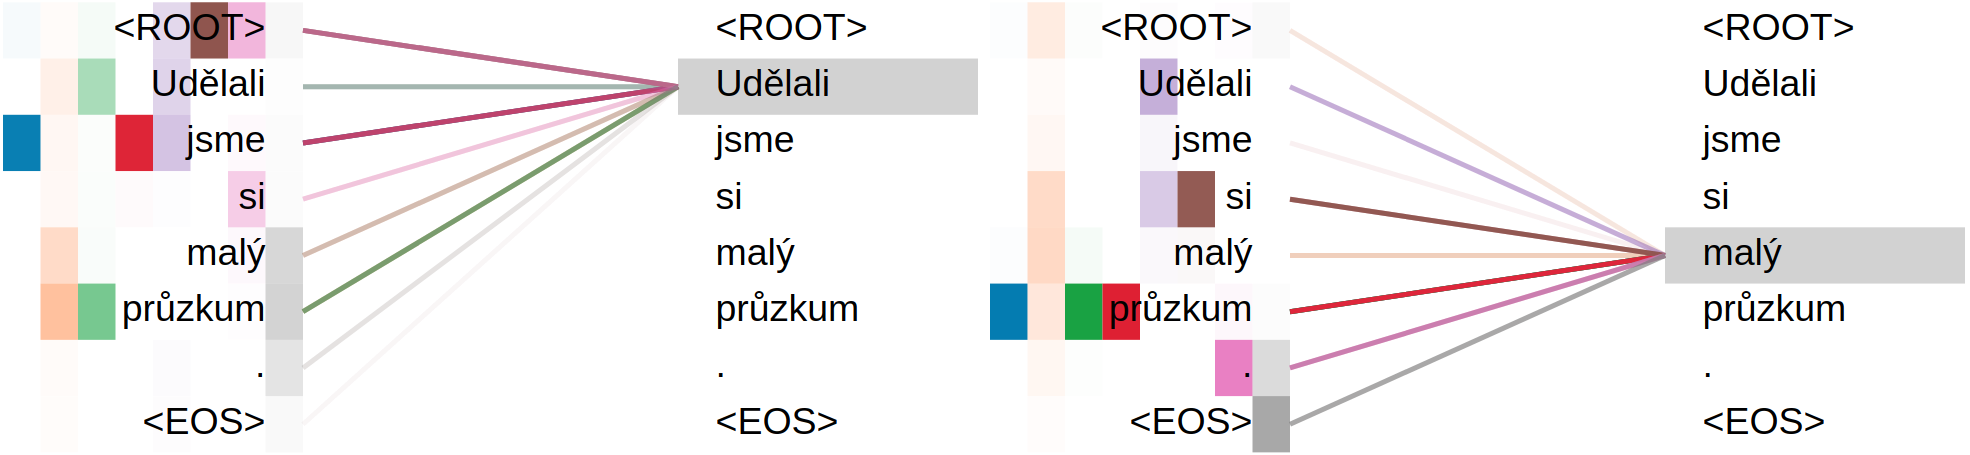
\includegraphics[width=\textwidth]{img/att-from4-l1.png}
        \caption{Layer 1}
    \end{subfigure}
    \begin{subfigure}[b]{0.9\textwidth}
        \centering
	    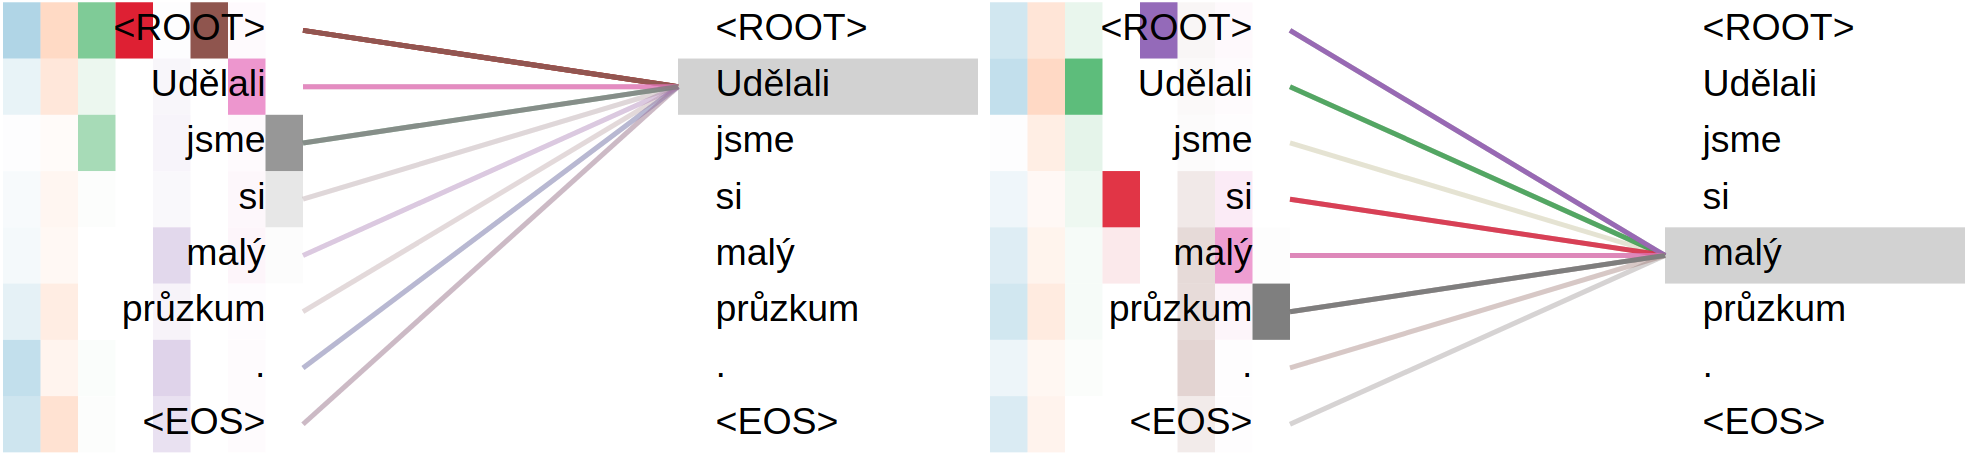
\includegraphics[width=\textwidth]{img/att-from4-l2.png}
        \caption{Layer 2}
    \end{subfigure}
    \begin{subfigure}[b]{0.9\textwidth}
        \centering
	    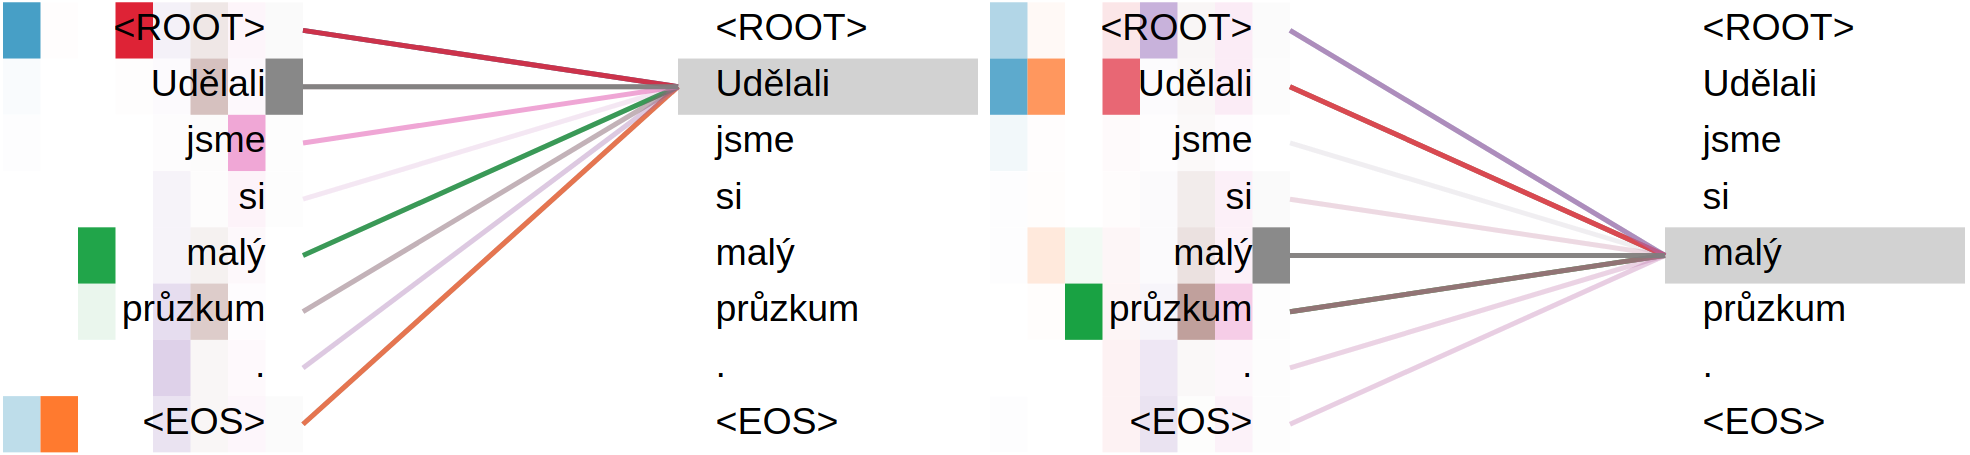
\includegraphics[width=\textwidth]{img/att-from4-l3.png}
        \caption{Layer 3}
    \end{subfigure}
    \begin{subfigure}[b]{0.9\textwidth}
        \centering
	    \frame{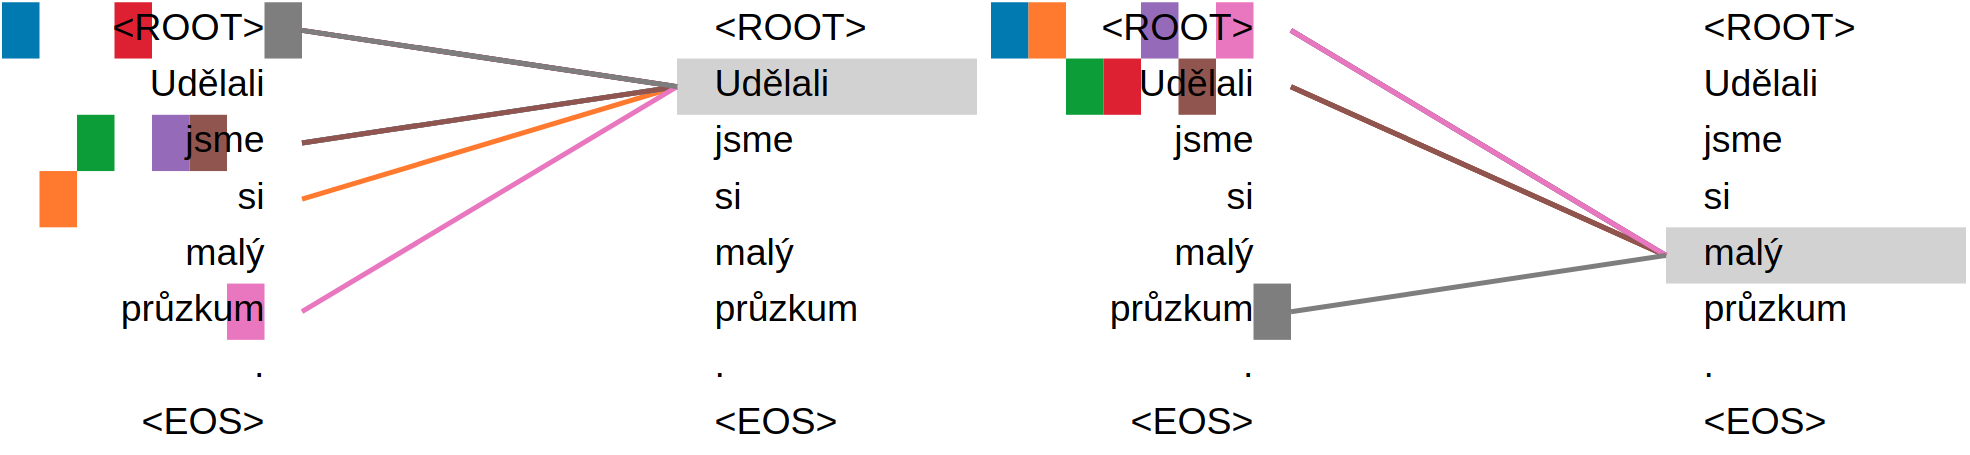
\includegraphics[width=\textwidth]{img/att-from4-l4.png}}
        \caption{Layer 4}
    \end{subfigure}
    \begin{subfigure}[b]{0.9\textwidth}
        \centering
	    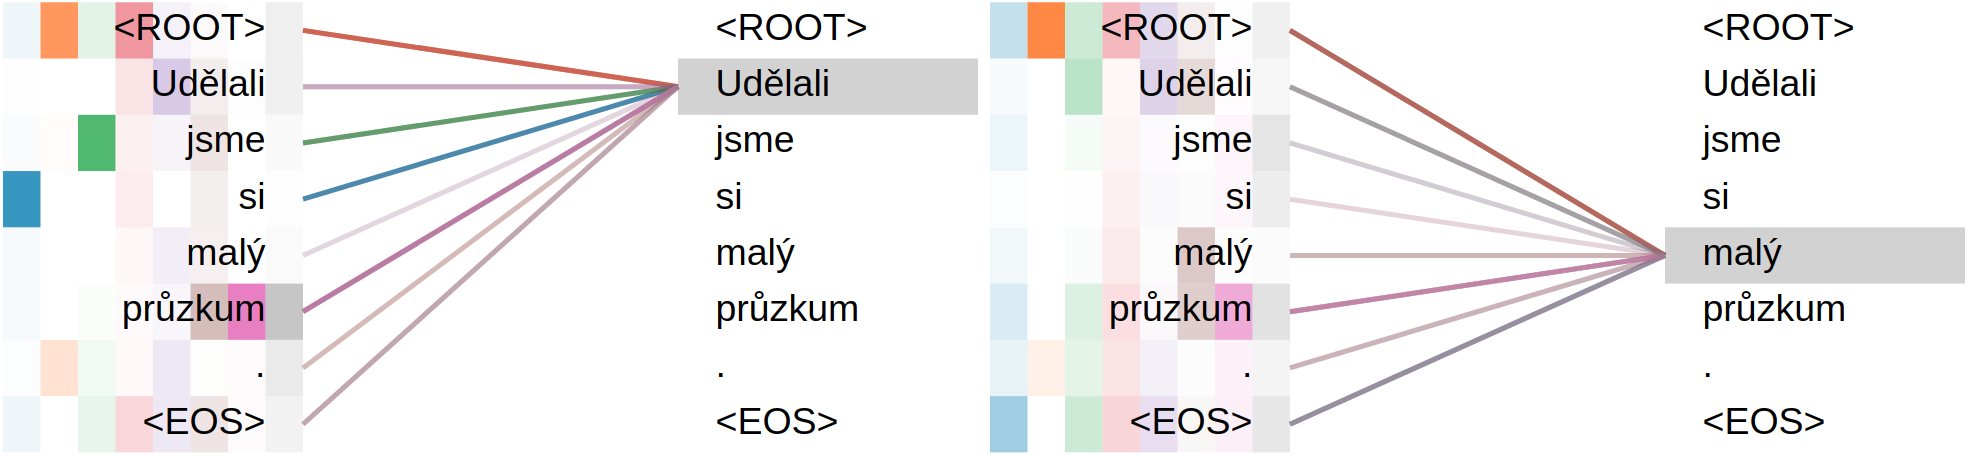
\includegraphics[width=\textwidth]{img/att-from4-l5.png}
        \caption{Layer 5}
    \end{subfigure}
    \caption{Visualization of the input-input attention in the \DepParse model in which syntax is demanded from the encoder's layer 4.}
    \label{fig:att-from4}
\end{figure}


\section{Training Speed}
\label{result-speed}

\begin{figure}[t]
    \centering
    \begin{tikzpicture}
        \begin{axis}[
        height=12cm, width=9cm, grid=major,
        xbar, xmin=0,
        xlabel={Percentage \%},
        symbolic y coords={
            {Transformer base},
            {Transformer relative},
            {TreeDistance, max 5},
            {(base) + TreeDistance, max 5},
            {(relative) + TreeDistance, max 5},
            {TreeTraversal},
            {(relative) + TreeTraversal},
            {(base) + SpecPOS},
            {(relative) + SpecPOS},
            {(base) + SpecDep},
            {(relative) + SpecDep},
            {DepParse (average)},
            {DiagonalParse (average)}
        },
        ytick=data,
        % nodes near coords, nodes near coords align={horizontal},
        ytick=data,
        ]
        \addplot coordinates {
            (100,{Transformer base})
            (111,{Transformer relative})
            (170,{TreeDistance, max 5})
            (196,{(base) + TreeDistance, max 5})
            (300,{(relative) + TreeDistance, max 5})
            (189,{TreeTraversal})
            (300,{(relative) + TreeTraversal})
            (100,{(base) + SpecPOS})
            (103,{(relative) + SpecPOS})
            (100,{(base) + SpecDep})
            (107,{(relative) + SpecDep})
            (113,{DepParse (average)})
            (110,{DiagonalParse (average)})
        };
        \end{axis}
    \end{tikzpicture}
    \caption{Training time to reach 250000 steps on a single GPU nVidia GTX 1080Ti (relative to the \transformerbase).}
    \label{fig:training-speed}
\end{figure}

Having proven that the \transformer NMT model has already captured the dependency syntax, our joint models derived from the \transformer were trained in a comparable time with the single-task \transformerbase.

Training time (including internal evaluation each 1000 steps) to reach 250,000 steps for the \transformerbase is 1 days, 3 hours, 48 minutes on a single GPU nVidia GTX 1080Ti.
On average, our joint dependency parsing and translation model \DepParse took only 13\% longer than the \transformerbase with significant improvement in translation task. \cref{fig:training-speed} also reveals the same for joint diagonal parsing and translation model \DiagonalParse, which took 10\% more time to train.

The encoder's enriched models with specialized attention heads are nearly identical to \transformerbase and \transformerrel.
The \SpecPOS models derived from \transformerbase and from \transformerrel took no extra time comparing to those baselines.
This is also applied to the \SpecDep models. 
However, they are different from the \SpecPOS models that they brought considerable improvements.

While having achieved similar results in translation task, the other set of methods enriching the encoder consumed more time to train.
In detail, the \TreeDistance with maximum distance of 5 consumed 70\% more of the time needed to train \transformerbase, while \TreeTraversal required 89\% more.
When combining with the positional encoding, the \TreeDistance, max 5 took 96\% more to train, but this cost brought significant improvement over both \transformerbase and \transformerrel.
Finally, the total training time for the \TreeDistance, max 5 and the \TreeTraversal when being combined with the relative position are 300\% of the \transformerbase's training time (+200\%). This huge amount of surplus training time were shown to yield improvements as well (\cref{result-enriching}).

The extra amount of training time required by the family of \TreeDistance and \TreeTraversal models were caused by the tree distance and tree encoding matrix's generation, and also the multiplication of these matrices with the key and query vectors.
These computations are quadratic in the length of the input sentence and need to be done on every attention layers of the encoder.
Interestingly, the joint models consumed only a little more time than \transformerbase but brought improvements on translation tasks and good parsing accuracy.
This result was obtained by the fact that our joint models do not add a separate parser on top of the encoder as the common practice in multi-task models, but use the self-attention matrix as the near output layer, then top it with an $argmax$ layer for the head selection.


\chapter*{Conclusion}
\addcontentsline{toc}{chapter}{Conclusion}

In this thesis, we proposed several methods to exploit the sentence structure in NMT by manipulation of the attention mechanism.
While aiming at the same goal, the previous works focused mostly on the \seq2seq model utilizing RNNs, we explore the state-of-the-art Transformer model which was built entirely on the attention mechanism.
We speculate that this mechanism makes it easier for us to direct the neural network's behavior with additional syntactic information, e.g. the dependency tree.

We evaluated the models on Czech-to-English and German-to-Czech translations, both in relatively large data setting, against \transformerbase (positional encoding) and \transformerrel (relative position).

The first set of methods attempted to enrich the encoder with source-side dependency tree.
First, we replaced the positional encoding and relative position with our proposed tree distance and tree traversal encoding.
BLEU scores of these models showed no improvement over the baselines.
However, combining our proposals with the baselines reported +0.5 to +0.8 BLEU against both baselines.
In addition, experiment results suggested that tree traversal works better than tree distance.

In this direction, we also proposed a specialized attention layer.
The difference between this and the standard attention layer is that the key and query come from an additional input sequence containing linguistic information, either POS tags or dependency labels.
The specialized POS head did not bring any improvement over baselines.
On the other hand, specialized dependency head brought +0.95 to +1.06 compared against the baselines without this modification.

We further invented a novel component of the Transformer model for sentence structure parsing by promoting the interpretation of self-attention as dependency syntax, and showed that the Transformer model can be used as a precise parser.
As suggested by the results, constraining self-attention to both true dependency as well as a simple diagonal matrix helped translation task at insignificant extra cost.
The best model of \DepParse and \DiagonalParse achieved +1.35 and +1.48 BLEU improvements, respectively. 
The models also performed well on parsing tasks.
\DepParse's best model achieved 91.56 UAS on the auto-generated treebanks, while \DiagonalParse, unsurprisingly, obtained 99.99\% accuracy.
Furthermore, \DepParse model performance is comparable to the referential parsers that were used to provide the parallel corpus with dependency trees.

To conclude our findings for the two main research questions of this thesis, it is clear from the results that enriching the \transformer with sentence structure can help.
However, the \transformer model is in fact able to capture this type of linguistic information already on its own and the guidance through multi-task learning is needed only as a small push towards trees following the annotation rules.


% Future works

\section*{Future Work}

While this thesis has explored various possibilities of exploiting sentence structure in NMT, we believe that there is still a vast room for improvements, which includes but is not limited to:

\paragraph{Fine-tuning the \DepParse model with gold-annotated data.}
Leveraging the self-attention weights to do both parsing and translation outperformed the baseline translation model and was comparable to referential parsers.
However, our model was trained on a synthetic treebank.
Hence, we could also try to fine-tune our model with the gold annotated treebank, which we believe should lead to a better parsing performance.

\paragraph{Examining dependency on subword units.}
In this thesis, we were working on the word level, without subword units, for an easier alignment with the dependency structure of the sentence.
Hence, all of the models had to face a serious out-of-vocabulary problem.
We would like to examine various methods to push the dependency relation beyond the word level, to subword level.
With that, we will be able to compare our proposed methods against the state-of-the-art translation models.


%%% Bibliography
%%% Bibliography (literature used as a source)
%%%
%%% We employ bibTeX to construct the bibliography. It processes
%%% citations in the text (e.g., the \cite{...} macro) and looks up
%%% relevant entries in the bibliography.bib file.
%%%
%%% The \bibliographystyle command selects, which style will be used
%%% for references from the text. The argument in curly brackets is
%%% the name of the corresponding style file (*.bst). Both styles
%%% mentioned in this template are included in LaTeX distributions.

\bibliographystyle{plainnat}    %% Author (year)
% \bibliographystyle{unsrt}     %% [number]

\renewcommand{\bibname}{Bibliography}

%%% Generate the bibliography. Beware that if you cited no works,
%%% the empty list will be omitted completely.

\bibliography{bibliography}

%%% If case you prefer to write the bibliography manually (without bibTeX),
%%% you can use the following. Please follow the ISO 690 standard and
%%% citation conventions of your field of research.

% \begin{thebibliography}{99}
%
% \bibitem{lamport94}
%   {\sc Lamport,} Leslie.
%   \emph{\LaTeX: A Document Preparation System}.
%   2nd edition.
%   Massachusetts: Addison Wesley, 1994.
%   ISBN 0-201-52983-1.
%
% \end{thebibliography}


%%% Figures used in the thesis (consider if this is needed)
\listoffigures

%%% Tables used in the thesis (consider if this is needed)
%%% In mathematical theses, it could be better to move the list of tables to the beginning of the thesis.
\listoftables

%%% Abbreviations used in the thesis, if any, including their explanation
%%% In mathematical theses, it could be better to move the list of abbreviations to the beginning of the thesis.
\chapwithtoc{List of Abbreviations}

\begin{table}[h]
    \begin{tabular}{p{2cm}l}
        BLEU & bilingual evaluation understudy \\
        cs & Czech \\
        cs2en & Czech-to-English \\
        de & German \\
        de2cs & German-to-Czech \\
        en & English \\
        GPU & graphical processing unit \\
        MT & machine translation \\
        NMT & neural machine translation \\
        PDT & Prague Dependency Treebank \\
        POS & part of speech \\
        RBMT & rule-based machine translation \\
        ReLU & rectified linear unit \\
        RNN & recurrent neural network \\
        seq2seq & sequence-to-sequence \\
        SMT & statistical machine translation \\
        T2T & Tensor2Tensor \\
        UD & Universal Dependencies \\
        WMT & Workshop on Machine Translation \\
    \end{tabular}
\end{table}

%%% Attachments to the master thesis, if any. Each attachment must be
%%% referred to at least once from the text of the thesis. Attachments
%%% are numbered.
%%%
%%% The printed version should preferably contain attachments, which can be
%%% read (additional tables and charts, supplementary text, examples of
%%% program output, etc.). The electronic version is more suited for attachments
%%% which will likely be used in an electronic form rather than read (program
%%% source code, data files, interactive charts, etc.). Electronic attachments
%%% should be uploaded to SIS and optionally also included in the thesis on a~CD/DVD.
%%% Allowed file formats are specified in provision of the rector no. 72/2017.
% \appendix
% \chapter{Attachments}

% \section{First Attachment}

% \openright
\end{document}
